\documentclass[11pt,a5paper,twoside,bahasa,listof=nochaptergap]{book}
\usepackage[tmargin=2.5cm,bmargin=2.5cm,lmargin=2.5cm,rmargin=2.0cm]{geometry}
\setcounter{secnumdepth}{5}
\usepackage[titletoc]{appendix}
\usepackage{csvsimple,longtable,booktabs}
\usepackage{listings}
\usepackage{diagbox}
\usepackage{csquotes}
\usepackage{tikz}
\usepackage{amsmath}
\usepackage[titles]{tocloft}

\begingroup
\makeatletter
\let\newcounter\@gobble\let\setcounter\@gobbletwo
\globaldefs\@ne \let\c@loldepth\@ne
\newlistof{listings}{lol}{\lstlistlistingname}
\newlistentry{lstlisting}{lol}{0}
\makeatother
\endgroup

\cftsetindents{lstlisting}{0in}{1.3in}

\lstset{ %
	numbers=left,
	xleftmargin=2mm,
	xrightmargin=2mm,
	frame=single,
	framesep=2mm,
	basicstyle=\footnotesize\ttfamily,
	framexleftmargin=2em,
	captionpos=b,
	belowcaptionskip=4pt,
	frame=single,
	breaklines=true,
	postbreak=\raisebox{0ex}[0ex][0ex]{\ensuremath{\color{red}\hookrightarrow\space}}
}
\usepackage{color, colortbl}
\definecolor{LightCyan}{rgb}{0.88,1,1}
\usepackage{rotating}
\usepackage{mdframed}
\usepackage{clrscode3e}
\usepackage[parfill]{parskip}
\usepackage{graphics}
\usepackage{fontspec}
\setsansfont{Trebuchet MS}
\setmainfont{Times New Roman}
\setmonofont{Courier New}
\usepackage{tocbibind}
\usepackage{enumitem}
\usepackage{pdflscape}
\usepackage{minted}
\usepackage{multirow}
\usepackage{graphicx}
\usepackage[verbose]{wrapfig}
\usepackage{changepage}
\usepackage{eso-pic}
\usepackage{ragged2e}
\usepackage{xesearch}
\usepackage[bahasa]{babel}
\usepackage[breaklinks=true]{hyperref}
\usepackage[font=small]{caption}
\usepackage{enumitem}
\setlist{nolistsep}
\usepackage{float}
\usepackage{longtable}
\usepackage{array,etoolbox}
\usepackage{amssymb}
\preto\tabular{\setcounter{magicrownumbers}{0}}
\preto\longtable{\setcounter{magicrownumbers}{0}}
\newcounter{magicrownumbers}
\newcommand\rownumber{\stepcounter{magicrownumbers}\arabic{magicrownumbers}}

\newcommand\nc[1]{%
	\multicolumn{1}{c}{#1}%
}

\newcommand\tab[1][1cm]{\hspace*{#1}}

\usepackage{setspace}
\singlespacing
\usepackage{fancyhdr}
\fancyhf{}
\renewcommand{\headrulewidth}{0pt}
\lhead[\thepage]{}
\rhead[]{\thepage}
\pagestyle{fancy}

\usepackage{titlesec}
\titleformat{\chapter}[display]{\filcenter\fontsize{11}{11}\bfseries}{\chaptername \ \thechapter}{0pt}{\filcenter\fontsize{11}{11}\bfseries\uppercase}
\titlespacing*{\chapter}{0pt}{-0.5cm}{40pt}
\titlespacing*{\section}{0pt}{11pt}{0pt}
\titlespacing*{\subsection}{0pt}{11pt}{0pt}
\titlespacing*{\subsubsection}{0pt}{11pt}{0pt}
\titleformat*{\section}{\fontsize{11}{11}\bfseries}
\titleformat*{\subsection}{\fontsize{11}{11}\bfseries}
\titleformat*{\subsubsection}{\fontsize{11}{11}\bfseries}


\addto\captionsbahasa{%
	\renewcommand\bibname{DAFTAR PUSTAKA}%
	\renewcommand\contentsname{DAFTAR ISI}%
	\renewcommand\listtablename{DAFTAR TABEL}%
	\renewcommand\listfigurename{DAFTAR GAMBAR}%
	\renewcommand\chaptername{BAB}%
}

\setlength{\parindent}{1cm}

\usepackage{chngcntr}
\renewcommand{\lstlistingname}{Kode Sumber}
\renewcommand{\lstlistlistingname}{DAFTAR KODE SUMBER}
\renewcommand*\thechapter{\arabic{chapter}}
\renewcommand\cftlstlistingpresnum{Kode Sumber }
\newcommand{\var}[2]{\newcommand{#1}{#2}}
\var{\judul}{Rancang Bangun Sistem Berbasis Internet of Things "EasyMeeting" Menggunakan NodeMCU dan Telegram Bot Untuk Meningkatkan Efisiensi Persiapan Ruang Rapat }
\var{\perusahaan}{PT Telekomunikasi Indonesia Tbk (Telkom) STO Gambir }
\var{\alamatPerusahaan}{Jalan Medan Merdeka Selatan No. 12 Jakarta Pusat }
\var{\kodePos}{10110 }
\var{\periode}{02 Januari-02 Februari 2018 }

\var{\namaPenulisSatu}{Hafara Firdausi }
\var{\nrpPenulisSatu}{5115 100 043 }
\var{\namaPenulisDua}{Nahda Fauziyah Zahra }
\var{\nrpPenulisDua}{5115 100 141 }
\var{\departemen}{Informatika }
\var{\fakultas}{Teknologi Informasi dan Komunikasi }
\var{\prodi}{S-1 }
\var{\perguruanTinggi}{Institut Teknologi Sepuluh Nopember }
\var{\pembimbingDept}{Radityo Anggoro S.Kom, M.Sc }
\var{\nipPembimbingDept}{19841016 200812 1 002 }
\var{\pembimbingLap}{Doddy Nur Pratomo }
\var{\nipPembimbingLap}{790101 }
\var{\jabatanPembimbingLap}{Unit \textit{Service Platform Development} }

\var{\sistem}{Sistem Berbasis \textit{Internet of Things} "EasyMeeting"}
\var{\namaSistem}{sistem berbasis \textit{Internet of Things} "EasyMeeting" }

\usepackage{caption}
\captionsetup[table]{labelsep=space}
\captionsetup[figure]{labelsep=space}
\captionsetup[lstlisting]{labelsep=space}

\setlength\cftparskip{-2pt}
\setlength\cftbeforechapskip{0pt}
\setlength{\lineskip}{0pt}

% Pemenggalan Tambahan
%english
%\hyphenation{ver-tex}
%\hyphenation{bridge}
%\hyphenation{block}
%\hyphenation{weight}
%\hyphenation{dis-joint}
%\hyphenation{par-ent}
%\hyphenation{root}
%\hyphenation{node}
%\hyphenation{set}
%\hyphenation{bridge-block}
%\hyphenation{con-nected}
%\hyphenation{com-po-nent}
%\hyphenation{undi-rected}
%\hyphenation{di-rected}
%\hyphenation{par-tially}
%\hyphenation{fully}
%\hyphenation{query}
%\hyphenation{dataset}

%bahasa
\hyphenation{me-nge-ta-hui}
\hyphenation{me-nya-ta-kan}
\hyphenation{meng-i-ni-si-al-i-sa-si}
\hyphenation{meng-gu-na-kan}
\hyphenation{me-la-ku-kan}
\hyphenation{me-li-bat-kan}
\hyphenation{permasalahan}

\makeatletter
\def\emptypage@emptypage{%
	\begin{center}
		\emph{Halaman ini sengaja dikosongkan}
	\end{center}
	\newpage%
}%
\def\cleardoublepage{%
	\clearpage%
	\if@twoside%
	\ifodd\c@page%
	% do nothing
	\else%
	\emptypage@emptypage%
	\fi%
	\fi%
}%
\makeatother
\raggedbottom


\renewcommand{\cftchapleader}{\cftdotfill{\cftdotsep}}
\renewcommand{\cftchappresnum}{BAB }
\renewcommand{\cfttabpresnum}{Tabel }
\cftsetindents{tab}{1em}{4.7em}
\renewcommand{\cftfigpresnum}{Gambar }
\cftsetindents{fig}{1em}{5.5em}

\cftsetindents{chapter}{0em}{3.6em}      % set amount of 
\cftsetindents{section}{2em}{2em}

\renewcommand{\thechapter}{\Roman{chapter}}
\renewcommand{\thesection}{\arabic{chapter}.\arabic{section}}
\renewcommand{\thesubsection}{\arabic{chapter}.\arabic{section}.\arabic{subsection}}
\renewcommand{\thefigure}{\arabic{chapter}.\arabic{figure}}
\renewcommand{\thetable}{\arabic{chapter}.\arabic{table}}

\newcommand{\insertfigure}{\begin{figure}\caption{A figure}\end{figure}}
\usepackage{etoolbox}% http://ctan.org/pkg/etoolbox
\makeatletter
% \patchcmd{<cmd>}{<search>}{<replace>}{<succes>}{<failure>}
\patchcmd{\@chapter}{\addtocontents{lof}{\protect\addvspace{10\p@}}}{}{}{}
\patchcmd{\@chapter}{\addtocontents{lot}{\protect\addvspace{10\p@}}}{}{}{}
\makeatother

\makeatletter
\g@addto@macro\appendix{%
	\addtocontents{toc}{%
		\protect\renewcommand{\protect\cftchappresnum}{}%
	}%
}
\makeatother


\renewcommand{\cftchapaftersnumb}{\hspace{0em}}

% Table caption above table
\floatstyle{plaintop}
\restylefloat{table}

% Centering table caption
\usepackage[justification=centering]{caption}
% Prevent hyphenation
\usepackage[none]{hyphenat}

\usepackage{mfirstuc}

\usepackage{tikz}

\begin{document} \sloppy
	% To prevent lstlisting from roman numbering
	\renewcommand{\thelstlisting}{\arabic{chapter}.\arabic{lstlisting}}
	\renewcommand{\theequation}{\arabic{chapter}.\arabic{equation}}
	
	% To remove spacing between chapter in list of figure and list of table
	\addtocontents{lof}{\protect\renewcommand*\protect\addvspace[1]{}}
	\addtocontents{lot}{\protect\renewcommand*\protect\addvspace[1]{}}
	
	% \setlength{\abovecaptionskip}{-12.75pt}
	
	\title {\judul}
	\author {\penulis}
	
	\frontmatter
	\addcontentsline{toc}{chapter}{SAMPUL}
	\newpage
	\newgeometry{top=6cm,left=2cm,bottom=2cm}

	\sffamily
	\thispagestyle{empty}
	\color{white}
	{ \noindent KERJA PRAKTIK - KI141330 }\\[25pt] 
	{\large\textbf{\MakeUppercase{\judul}}} \\[18pt]
	{\small{\perusahaan}} \\
	{\small{\alamatPerusahaan}} \\
	{\small{Periode: \periode}} \\
	\\
	\\
	\\
	Oleh:\\[5pt]
	\begin{tabular}{ll}
		\MakeUppercase{\namaPenulisSatu} & \hspace{20pt} NRP \nrpPenulisSatu \\
		\MakeUppercase{\namaPenulisDua} & \hspace{20pt} NRP \nrpPenulisDua \\
	\end{tabular}\\[10pt]
	Dosen Pembimbing Departemen \\
	\pembimbingDept \\[10pt]
	Dosen Pembimbing Lapangan \\
	\pembimbingLap \\[10pt]
	DEPARTEMEN \MakeUppercase{\departemen} \\
	Fakultas \fakultas \\
	{\perguruanTinggi} \\
	Surabaya, 2018
	\AddToShipoutPictureBG*{
\includegraphics[width=\paperwidth,height=\paperheight]{sampul/sampul.png}}
	\rmfamily
	\normalsize
	\restoregeometry
	\color{black}
	\cleardoublepage
	
\newpage
	\newgeometry{top=6cm,left=2cm,bottom=2cm}

	\sffamily
	\thispagestyle{empty}
	{ \noindent KERJA PRAKTIK - KI141330 }\\[25pt] 
	{\large\textbf{\MakeUppercase{\judul}}} \\[18pt]
	{\small{\perusahaan}} \\
	{\small{\alamatPerusahaan}} \\
	{\small{Periode: \periode}} \\
	\\
	\\
	\\
	Oleh:\\[5pt]
	\begin{tabular}{ll}
		\MakeUppercase{\namaPenulisSatu} & \hspace{20pt} NRP \nrpPenulisSatu \\
		\MakeUppercase{\namaPenulisDua} & \hspace{20pt} NRP \nrpPenulisDua \\
	\end{tabular}\\[10pt]
	Dosen Pembimbing Departemen \\
	\pembimbingDept \\[10pt]
	Dosen Pembimbing Lapangan \\
	\pembimbingLap \\[10pt]
	DEPARTEMEN \MakeUppercase{\departemen} \\
	Fakultas \fakultas \\
	{\perguruanTinggi} \\
	Surabaya, 2018
	\AddToShipoutPictureBG*{
\includegraphics[width=\paperwidth,height=\paperheight]{sampul/sampulWhite.png}}
	\rmfamily
	\normalsize
	\restoregeometry
	\color{black}
	\cleardoublepage

	\addcontentsline{toc}{chapter}{LEMBAR PENGESAHAN}
	\newpage
	\thispagestyle{plain}
	\begin{centering}
		\textbf{\MakeUppercase{\judul}} \\[20pt]
		\textbf{\large{KERJA PRAKTIK}} \\[20pt]
		
		Oleh: \\
		\begin{tabular}{ll}
			\MakeUppercase{\namaPenulisSatu} & \hspace{20pt} NRP \nrpPenulisSatu \\
			\MakeUppercase{\namaPenulisDua} & \hspace{20pt} NRP \nrpPenulisDua \\
		\end{tabular}\\[30pt]
	\end{centering}

	{\noindent Disetujui oleh Pembimbing Kerja Praktik:}\\[30pt]         
	\pembimbingDept \hfill \hfill .......................... \\
	NIP: \nipPembimbingDept \hfill \hfill (Pembimbing Departemen) \\[50pt]
	{\noindent \pembimbingLap  \hfill \hfill ...........................}  \\
	\jabatanPembimbingLap \hfill \hfill (Pembimbing Lapangan) \\[20pt] 

	\begin{centering}
		\textbf{SURABAYA} \\*
		\textbf{FEBRUARI 2018} \\*
	\end{centering}
	\cleardoublepage
	\addcontentsline{toc}{chapter}{ABSTRAK}
\thispagestyle{plain}
\begin{centering}
	\textbf{\MakeUppercase{\judul}}
\end{centering} \\[20pt]
\begin{tabular}{ll}
	Nama Mahasiswa  &: \MakeUppercase{\namaPenulisSatu} \\
	NRP &: \nrpPenulisSatu \\
	Nama Mahasiswa  & : \MakeUppercase{\namaPenulisDua} \\
	NRP &: \nrpPenulisDua \\
	Departemen  &: Departemen \departemen FTIK-ITS \\
	Pembimbing Departemen  &: \pembimbingDept \\
	Pembimbing Lapangan  &: \pembimbingLap
\end{tabular} \\[10pt]
\begin{center}
	\textbf{ABSTRAK}
\end{center}
\indent\indent Dengan kemajuan teknologi di zaman sekarang, BRI menjadi satu-satunya Bank di dunia yang memiliki satelit sendiri. Oleh karenanya, dilakukan relokasi ATM untuk diarahkan langsung menuju satelit milik BRI. Untuk keberlangsungan kegiatan relokasi ATM, diperlukan sebuah sistem informasi sebagai wadah kontrol pengerjaan proyek relokasi ATM BRI.
\indent Pada laporan kerja praktik ini, penulis akan menguraikan secara garis besar pengerjaan aplikasi \textit{Monitoring} SIK yang menggunakan bahasa pemrograman HTML, CSS, JavaScript serta PHP.\\
\indent Berdasarkan hasil uji coba dan evaluasi menunjukkan bahwa aplikasi \textit{Monitoring} SIK yang dibuat telah berhasil memenuhi kebutuhan informasi yang dibutuhkan dalam memantau pengerjaan proyek relokasi. \\[10pt]
\textbf{Kata Kunci: \textit{Internet of Things}, SIK, relokasi}


\cleardoublepage

	\chapter{KATA PENGANTAR}
\indent\indent Puji syukur kami panjatkan ke hadirat Allah SWT atas segala karunia-Nya, sehingga kami dapat menyelesaikan penyusunan buku laporan kerja praktik dengan judul :
\begin{center}
	\textbf{\judul}
\end{center}

Melalui buku laporan ini, kami juga ingin menyampaikan terima kasih yang sedalam-dalamnya kepada orang-orang yang telah membantu kami, baik secara langsung maupun tidak langsung, dalam penyelesaian kerja praktik hingga penyusunan buku laporan, antara lain:
\begin{enumerate}
\item Kedua orang tua dan keluarga penulis.
\item Bapak \pembimbingDept selaku koordinator kerja praktik, sekaligus dosen pembimbing kerja praktik selama kerja praktik berlangsung.
\item Bapak \pembimbingLap selaku pembimbing lapangan di PT Telekomunikasi Indonesia selama kerja praktik berlangsung.
\item Seluruh \jabatanPembimbingLap (SPD) Divisi IT PT Telekomunikasi Indonesia, serta tim WSO2 Sigma yang telah menemani, membantu, dan memberikan kami ilmu yang berguna selama kerja praktik berlangsung. 
\item Teman-teman selama kerja praktik, Adam Alfian dan Faturochman Pranacahya, yang telah menjadi salah satu sumber semangat untuk melaksanakan kerja praktik.
\end{enumerate}
\indent\indent Kami menyadari sepenuhnya bahwa masih banyak kekurangan dalam pelaksanaan kerja praktik maupun penyusunan buku laporan ini. Namun, kami berharap buku laporan ini dapat bermanfaat untuk menambah wawasan pembaca dan dapat menjadi sumber referensi.\\

\hfill Surabaya, Februari 2018 \\ 

\begin{flushright}
\hfill{Penulis} 
\end{flushright}
\cleardoublepage

	\tableofcontents
	\cleardoublepage
	\listoftables
	\cleardoublepage
	\listoffigures
	\cleardoublepage
	\lstlistoflistings
	\cleardoublepage
	
	\mainmatter
	\chapter{PENDAHULUAN}

\section{Latar Belakang}
\tab PT Telkom Indonesia (Persero) Tbk (Telkom) adalah Badan Usaha Milik Negara (BUMN) yang bergerak di bidang jasa layanan teknologi informasi dan komunikasi (TIK) dan jaringan telekomunikasi di Indonesia. Misi Telkom adalah "\textit{Lead Indonesian Digital Innovation and Globalization}",\cite{Profil Telkom} yang artinya Telkom harus memimpin inovasi digital di Indonesia, salah satunya adalah inovasi teknologi \textit{Internet of Things} yang belum banyak diimplementasikan di Indonesia. \\
\tab \textit{Internet of Things} (IoT) merupakan sebuah teknologi yang mampu mengubah perangkat menjadi sesuatu yang berharga, diantaranya untuk \textit{monitoring} dan analisis. Di Indonesia, teknologi IoT masih kalah dengan industri teknologi lainnya semacam \textit{e-commerce} dan teknologi finansial. Banyak hal yang menghambat pertumbuhan IoT di Indonesia, mulai dari kebijakan mengenai perangkat, data, hingga frekuensi penggunaan. Dari segi pemanfaatannya, IoT memiliki banyak peluang, baik untuk pengguna umum atau bisnis. Dari rilis yang dikeluarkan Hitachi, teknologi IoT akan menjadi tren global di tahun 2018.\cite{Perkembangan Industri Internet of Things di Indonesia Tahun 2017} \\
\tab Saat ini, Telkom sedang mengembangkan sebuah produk yang dapat mengimplementasikan \textit{server-side Internet of Things} (IoT) \textit{platform} bernama WSO2 IoT Server. Produk tersebut nantinya akan diperjualbelikan layaknya produk-produk Telkom yang lain, seperti IndiHome. Namun, Telkom harus menguji produk tersebut terlebih dahulu sebelum diluncurkan dan diperjualbelikan. \\
\tab Di sisi lain, Telkom merupakan sebuah perusahaan besar yang aktivitas para pegawainya tidak lepas dari kata "rapat". Rapat sudah menjadi bagian dari kehidupan sehari-hari karena ada banyak permasalahan yang harus didiskusikan dan juga sebagai media untuk melakukan \textit{sharing progress}. Namun, kami melihat persiapan rapat di Telkom kurang efisien. Ada banyak hal yang harus dilakukan, seperti menyalakan AC \textit{(Air Conditioner)}, menyalakan lampu, dan sebagainya, sehingga waktu dimulainya rapat menjadi molor. \\
\tab Dari beberapa permasalahan diatas, Telkom membutuhkan sebuah sistem yang dapat digunakan untuk mencoba produk baru Telkom, yaitu WSO2 IoT Server, sekaligus memiliki daya guna lebih, yakni untuk meningkatkan efisiensi persiapan ruang rapat di PT Telkom Indonesia. Oleh karena itu, kami menawarkan solusi dengan membangun sebuah sistem berbasis \textit{Internet of Things} yang bernama "EasyMeeting". Sistem ini memiliki konsep yang sama seperti \textit{Smart House}, yakni membuat sebuah ruangan pintar yang dapat dikendalikan menggunakan \textit{mobile phone}, \textit{device} yang dimiliki oleh hampir semua orang. \\
\tab Dengan adanya \namaSistem ini, diharapkan efisiensi rapat dan produktivitas di Telkom dapat meningkat. Sistem ini nantinya juga dapat digabungkan dengan sistem manajemen ruang rapat yang sudah ada di Telkom. \textit{EasyMeeting, meeting as easy as tapping!}  

\section{Tujuan}
\tab Tujuan dari pengerjaan kerja praktik ini adalah:
\begin{enumerate}
	\item Membangun sebuah sistem berbasis \textit{Internet of Things} yang dapat meningkatkan efisiensi persiapan ruang rapat di PT Telkom Indonesia sekaligus untuk menguji produk Telkom, WSO2 IoT Server.
	\item Membangun sebuah sistem berbasis \textit{Internet of Things} yang mudah dimengerti oleh pengguna dan dapat diakses dimana saja.
\end{enumerate}

\section{Manfaat}
\tab Manfaat yang diperoleh dari pengerjaan kerja praktik ini adalah:
\begin{enumerate}
	\item Meningkatkan efisiensi dan mempersingkat waktu persiapan ruang rapat di PT Telkom Indonesia, sehingga rapat dapat dimulai tepat waktu.
	\item Telkom dapat menguji produk barunya, yakni WSO2 IoT Server.
	\item Pegawai Telkom dapat mengontrol ruang rapat dengan mudah dan dimana saja.
	\item Menambah ilmu dalam pembuatan sistem berbasis \textit{Internet of Things} menggunakan teknologi-teknologi terbaru.
\end{enumerate}

\section{Rumusan Masalah}
\tab Rumusan masalah yang akan dibahas dalam pengerjaan kerja praktik ini adalah:
\begin{enumerate}
	\item Bagaimana membangun sebuah sistem berbasis \textit{Internet of Things} yang dapat meningkatkan efisiensi persiapan ruang rapat di PT Telkom Indonesia sekaligus untuk menguji produk Telkom, WSO2 IoT Server?
	\item Bagaimana membangun sebuah sistem berbasis \textit{Internet of Things} yang mudah dimengerti oleh pengguna dan dapat diakses dimana saja?
	
\end{enumerate}

\section{Lokasi dan Waktu Kerja Praktik}
\tab Lokasi pelaksanaan kerja praktik dilakukan di kantor \perusahaan dengan alamat \alamatPerusahaan - Daerah Khusus Ibukota Jakarta. Kami ditempatkan di Divisi \textit{Information Technology} (IT).\\
\tab Adapun kerja praktik dimulai pada tanggal 02 Januari 2018 hingga 02 Februari 2018, dengan hari kerja Senin sampai Jumat, pukul 08.00 sampai dengan pukul 17.00 WIB, dan sesuai dengan peraturan perusahaan.

\section{Metodologi}
\tab Tahapan metodologi dalam pengerjaan kerja praktik dapat dijabarkan sebagai berikut:
\begin{enumerate}
	\item \textbf{Perumusan Masalah}\\
	\tab Tahap pertama adalah merumuskan masalah. Untuk mengetahui permasalahan apa yang harus diselesaikan, diberikan penjelasan mengenai alasan mengapa sistem ini dibutuhkan. Dijelaskan pula secara rinci mengenai bagaimana alur sistem itu akan berjalan. Penjelasan yang diberikan oleh pembimbing kerja praktik menghasilkan beberapa catatan mengenai gambaran cara kerja sistem dan rincian kebutuhan sistem \textit{Internet of Things}. Setelah mendapatkan gambaran sistem, diskusi lebih lanjut dilakukan guna menentukan komponen-komponen \textit{microcontroller} yang dibutuhkan, bahasa pemrograman, dan \textit{platform} yang dipakai dalam pembuatan sistem.\\
	
	\item \textbf{Studi Literatur}\\
	\tab Setelah ditentukannya komponen-komponen \textit{microcontroller} yang dibutuhkan, bahasa pemrograman, dan \textit{platform} yang dipakai dalam pembuatan sistem, maka pada tahap ini dilakukan proses pencarian, pembelajaran, pengumpulan
	dan pemahaman informasi serta studi literatur lebih lanjut mengenai cara implementasinya dalam membangun sistem sesuai yang dibutuhkan.\\
	\tab Secara garis besar, untuk membuat \namaSistem digunakan beberapa mikrokontroler dan komponen elektronika, antara lain Arduino UNO, sensor suhu dan \textit{infrared}, \textit{breadboard}, serta \textit{jumper wires}; bahasa pemrograman C, Telegram Bot API dan WSO2 IoT Server, serta DBMS H2 atau SQLite sebagai penyimpanan data pegawai Telkom.\\
	
	\item \textbf{Analisis dan Perancangan Sistem}\\
	\tab Pada tahap ini akan dijelaskan tentang analisis serta perancangan sistem yang akan dibangun oleh penulis, berdasarkan studi literatur dan pembelajaran konsep teknologi dari perangkat lunak yang sudah ada.\\
	\tab Fungsi dari sistem \textit{Internet of Things} yang akan dibuat adalah untuk meningkatkan efisiensi persiapan ruang rapat, meliputi menyalakan dan mematikan lampu dan AC (\textit{Air Conditioner}), menyesuaikan suhu ruangan, serta menampilkan status ruangan. Sistem IoT dikendalikan melalui aplikasi Telegram, dengan memanfaatkan Telegram Bot API. Sistem IoT hanya bisa dikendalikan oleh pegawai internal Telkom saja, sehingga sistem ini juga dilengkapi dengan \textit{user authentication} dan \textit{database} pegawai Telkom.\\
	
	\item \textbf{Implementasi Sistem}\\
	\tab Implementasi merupakan tahap pembangunan rancangan. Pada tahap ini, penulis merealisasikan sesuai dengan analisis dan perancangan sistem yang telah dilakukan pada tahap sebelumnya.\\
	\tab Setidaknya ada empat pekerjaan utama yang dilakukan, yaitu desain antarmuka pengguna, yakni memanfaatkan Telegram Bot API; desain antarmuka perangkat keras, yakni merangkai komponen-komponen \textit{microcontroller} yang dibutuhkan, meliputi NodeMCU, sensor suhu dan \textit{infrared}, serta \textit{jumper wires}; desain fungsi-fungsi yang bekerja dalam sistem (\textit{back-end}), yakni menggunakan bahasa C/C++ dan Arduino IDE; dan desain \textit{database}. Pembangunan sistem dilakukan selama satu bulan.\\ 
	
	\item \textbf{Pengujian dan Evaluasi}\\
	\tab Pada tahap ini dilakukan uji coba pada sistem yang telah dibangun. Tahap ini dimaksudkan untuk menguji dan mengevaluasi fitur-fitur dalam sistem yang telah dibuat, apakah berjalan dengan baik dan sesuai dengan kebutuhan atau tidak. Kesesuaian sistem dengan kebutuhan akan menentukan keberhasilan dalam pengujian. Selain itu, pengujian dan evaluasi juga dimaksudkan untuk mencari masalah yang mungkin timbul, serta mencari solusi untuk membuat sistem menjadi lebih baik.\\
	
	\item \textbf{Kesimpulan dan Saran}\\
	\tab Pada tahap ini dilakukan penarikan kesimpulan berdasarkan hasil implementasi dan pengujian sistem, serta diberikan saran terkait dengan hasil evaluasi untuk mengembangkan sistem menjadi lebih baik lagi.
\end{enumerate}

\section{Sistematika Laporan}
\tab Laporan kerja praktik ini terdiri dari tujuh bab dengan rincian sebagai berikut:
\begin{enumerate}
	\item \textbf{Bab I: Pendahuluan}\\
	\tab Bab ini memaparkan mengenai garis besar kerja praktik yang meliputi latar belakang, tujuan, manfaat, rumusan masalah, lokasi dan waktu kerja praktik, metodologi dan sistematika laporan.\\
		
	\item \textbf{Bab II: Profil Perusahaan}\\
	\tab Bab ini berisi gambaran umum profil perusahaan tempat pelaksanaan kerja praktik, yakni PT Telekomunikasi Indonesia (Persero) Tbk (Telkom), mulai dari visi dan misi perusahaan, portofolio bisnis perusahaan, sejarah perusahaan, hingga divisi tempat kerja praktik dilakukan, yakni divisi \textit{Information Technology} (IT).\\
		
	\item \textbf{Bab III: Tinjauan Pustaka}\\
	\tab Bab ini berisi penjelasan tentang istilah-istilah atau dasar teori dari metode atau teknologi yang digunakan dalam menyelesaikan proyek kerja praktik.\\
		
	\item \textbf{Bab IV: Analisis dan Perancangan Sistem}\\
	\tab Pada bab ini dijelaskan mengenai analisis terhadap sistem dan pemaparan mengenai kebutuhan untuk perancangan sistem yang akan dibangun dan dikembangkan.\\
	
	\item \textbf{Bab V: Implementasi Sistem}\\
	\tab Bab ini berisi uraian tahap-tahap implementasi sistem.\\
		
	\item \textbf{Bab VI: Pengujian dan Evaluasi}\\
	\tab Bab ini berisi hasil uji coba dan evaluasi dari sistem yang telah dikembangkan selama pelaksanaan kerja praktik.\\
	
	\item \textbf{Bab VII: Kesimpulan dan Saran}\\	
	\tab Bab ini berisi kesimpulan dan saran yang didapat dari proses pelaksanaan kerja praktik.\\
\end{enumerate}

\cleardoublepage

	\chapter{PROFIL PERUSAHAAN}
\tab PT Telkom Indonesia (Persero) Tbk (Telkom) adalah Badan Usaha Milik Negara (BUMN) yang bergerak di bidang jasa layanan teknologi informasi dan komunikasi (TIK) dan jaringan telekomunikasi di Indonesia. Pemegang saham mayoritas Telkom adalah Pemerintah Republik Indonesia sebesar 52.09\%, sedangkan 47.91\% sisanya dikuasai oleh publik. Saham Telkom diperdagangkan di Bursa Efek Indonesia (BEI) dengan kode “TLKM” dan New York Stock Exchange (NYSE) dengan kode “TLK” \cite{profil-telkom}.

\section{Visi dan Misi Perusahaan}
\tab Seiring dengan perkembangan teknologi digital dan transformasi perusahaan, Telkom memiliki visi dan misi baru yang diberlakukan sejak 2016, yaitu:
\subsection{Visi Perusahaan}
\tab Visi Telkom adalah "\textit{Be the King of Digital in the Region}", yang artinya Telkom akan menjadi perusahaan yang unggul dalam bidang teknologi digital \textit{(king of digital)} di kawasan regional.
\subsection{Misi Perusahaan}
\tab Misi Telkom adalah "\textit{Lead Indonesian Digital Innovation and Globalization}", yang artinya Telkom akan memimpin inovasi digital dan globalisasi di Indonesia. Untuk mencapai misi tersebut, Telkom memiliki \textit{strategic objectives} "\textit{Top 10 Market Capitalization Telco in Asia-Pacific by 2020 and maintain its stronghold position}".\\
\tab TelkomGroup juga telah menyusun strategi korporasi guna menciptakan \textit{sustainable competitive growth} dan mendorong cita-cita Indonesia untuk menjadi kekuatan ekonomi digital terbesar di Asia Tenggara, yaitu:
	\begin{enumerate}
		\item \textit{Directional Strategy: Disruptive competitive growth}\\
		\tab Di tengah perubahan lingkungan industri yang sangat menantang, TelkomGroup yakin bahwa kapitalisasi pasar akan tumbuh secara signifikan. Ini dilakukan dengan cara memberikan nilai lebih kepada pelanggan melalui inovasi produk dan layanan, mendorong sinergi serta membangun ekosistem digital yang kuat baik di pasar domestik maupun internasional.
		\item \textit{Portfolio Strategy: Customer value through digital TIMES portfolio}\\
		\tab TelkomGroup berfokus pada portofolio digital TIMES \textit{(Telecommunication, Information, Media, Edutainment \& Services)} melalui penyediaan layanan yang nyaman dan konvergen sehingga memberikan nilai yang tinggi kepada pelanggan.
		\item \textit{Parenting Strategy: Strategic Control}\\
		\tab Untuk mendukung pertumbuhan bisnis secara efektif, TelkomGroup menerapkan pendekatan \textit{strategic control} untuk menyelaraskan unit bisnis, unit fungsional dan anak perusahaan agar proses dapat berjalan lebih terarah, bersinergi, dan efektif dalam mencapai tujuan perusahaan.
	\end{enumerate}

\section{Sejarah Perusahaan}
\tab Dalam perjalanan sejarahnya, Telkom telah melalui berbagai dinamika bisnis dan melewati beberapa fase perubahan, yakni:
\begin{enumerate}
	\item Kemunculan Telepon (1882)\\
	\tab Pada tahun 1856, pemerintah kolonial Belanda membangun telegraf elektromagnetik pertama yang menghubungkan Jakarta (Batavia) dan Bogor. Kemudian tahun 1882, kemunculan teknologi telepon menyaingi layanan pos dan telegraf. Pemerintah Belanda membentuk lembaga yang mengatur layanan pos dan telekomunikasi di Indonesia dengan nama Jawatan \textit{Post Telegraaf Telefoon} (PTT).\\
	\item Kelahiran Telkom (1965)\\
	\tab Pada tahun 1957, banyak perusahaan-perusahaan Belanda yang diakuisisi oleh Indonesia. Pemerintah Soekarno memiliki visi menjadikan seluruh perusahaan negara menjadi \textit{public corporation}. Pada tahun 1961, Jawatan PTT berubah nama menjadi Perusahaan Negara Pos dan Telekomunikasi (PN Postel).\\
	\tab Namun, seiring berkembangnya layanan telepon dan telex, pemerintah Indonesia mengeluarkan Peraturan Pemerintah No. 30 tanggal 6 Juli 1965 yang berisi pemisahan industri pos dan telekomunikasi dalam PN Postel menjadi PN Pos dan Giro serta PN Telekomunikasi.\\
	\tab Dengan pemisahan ini, setiap perusahaan dapat fokus untuk mengelola portofolio bisnisnya masing-masing. Terbentuknya PN Telekomunikasi ini menjadi cikal-bakal Telkom saat ini. Sejak tahun 2016, manajemen Telkom menetapkan tanggal 6 Juli 1965 sebagai hari lahir Telkom.\\
	\item Perumtel (1974)\\
	\tab Pada tahun 1974, PN Telekomunikasi berubah nama menjadi Perusahaan Umum Telekomunikasi Indonesia (Perumtel) yang menyelenggarakan jasa telekomunikasi nasional maupun internasional.\\
	\item PT Telekomunikasi Indonesia (1991)\\
	\tab Pada tahun 1991, Perumtel berubah bentuk menjadi Perseroan Terbatas (PT) dengan nama Telekomunikasi Indonesia (Telkom) berdasarkan Peraturan Pemerintah Nomor 25 Tahun 1991.\\
	\item Melakukan Penawaran Umum Perdana Saham Telkom (1995)\\
	\tab Pada tanggal 14 November 1995, dilakukan Penawaran Umum Perdana saham Telkom. Sejak itu saham Telkom tercatat dan diperdagangkan di Bursa Efek Jakarta (BEJ/JSX) dan Bursa Efek Surabaya (BES/SSX) (keduanya sekarang bernama Bursa Efek Indonesia (BEI/IDX), Bursa Efek New York (NYSE) (Diperdagangkan pada tanggal 14 Juli 2003) dan Bursa Efek London (LSE). Saham Telkom juga diperdagangkan tanpa pencatatan di Bursa Saham Tokyo. Jumlah saham yang dilepas saat itu adalah 933 juta lembar saham.\\
	\tab Sejak 16 Mei 2014, saham Telkom tidak lagi diperdagangkan di Bursa Efek Tokyo (TSE) dan pada 5 Juni 2014 di Bursa Efek London (LSE).\\
	\item Membeli Telkomsel (2001)\\
	\tab Tahun 2001, Telkom membeli 35\% saham Telkomsel dari PT Indosat sebagai bagian dari implementasi restrukturisasi industri jasa telekomunikasi di Indonesia yang ditandai dengan penghapusan kepemilikan bersama dan kepemilikan silang antara Telkom dan Indosat (duopoli).\\
	\item \textit{New Telkom} (2009)\\
	\tab Pada 23 Oktober 2009, Telkom meluncurkan \textit{"New Telkom"} ("Telkom baru") yang ditandai dengan penggantian identitas perusahaan.\\
	\item Beroperasi di Tujuh Negara (2013)\\
	\tab Telkom telah beroperasi di tujuh negara seperti Australia, Hong Kong, Macau, Timor Leste, Malaysia, Taiwan, dan Amerika Serikat.\\
	\item Meluncurkan Layanan 4G (2014)\\
	\tab Melalui anak perusahaan, Telkomsel, menjadi operator pertama yang meluncurkan layanan 4G secara komersial.
\end{enumerate}

\section{Divisi \textit{Information Technology}}
\tab Telkom memiliki struktur organisasi yang sangat besar dan kompleks, terdiri dari banyak divisi dan sub-divisi, salah satunya adalah divisi IT atau \textit{Information Technology}. Secara garis besar, divisi IT dibagi menjadi 2 bagian, yaitu \textit{Development} dan \textit{Operation}, dengan masing-masing bagian dipimpin oleh seorang \textit{Deputy EGM IT}. \textit{Deputy EGM IT Development} membawahi beberapa sub-divisi berikut:
\begin{enumerate}
	\item \textit{Enterprise \& Analytic Platform Development}
	\item \textit{BSS \& CEM Platform Development}
	\item \textit{OSS Platform Development}
	\item \textit{Service Platform Development}
	\item \textit{IT Planning \& Architecture}
\end{enumerate}
\tab Sedangkan \textit{Deputy EGM IT Operation} membawahi sub-divisi berikut:
\begin{enumerate}
	\item \textit{Enterprise \& Analytic Platform Operation}
	\item \textit{BSS \& CEM Platform Operation}
	\item \textit{OSS Platform Operation}
	\item \textit{Service Platform Operation}
	\item \textit{CFU/FU Support \& ITSM}
\end{enumerate}
\tab Kedua \textit{deputy} bekerja dibawah pimpinan seorang \textit{Executive General Manager Information Technology} yang langsung membawahi sub-divisi \textit{General Affair}.\\
\tab Pada kesempatan kerja praktik ini, kami ditempatkan di sub-divisi \textit{Service Platform Development} (SPD) pada unit \textit{SOA Platform Development}.

\cleardoublepage
	\chapter{TINJAUAN PUSTAKA}
\section{\textit{Internet of Things}}
\tab \textit{Internet of Things} (IoT) adalah sebuah konsep komputasi yang menggambarkan sebuah gagasan tentang objek fisik sehari-hari yang terhubung ke internet dan mampu mengidentifikasi diri mereka ke perangkat lain. Istilah ini erat diidentifikasi oleh RFID sebagai metode komunikasi antar objek tanpa melibatkan interaksi manusia ke manusia atau manusia ke komputer, termasuk teknologi sensor, \textit{wireless}, atau \textit{QR codes}. IoT telah berkembang dari konvergensi teknologi nirkabel, \textit{micro-electromechanical systems} (MEMS), dan internet.\\
\tab IoT adalah signifikan, karena sebuah objek dapat merepresentasikan dirinya secara digital menjadi sesuatu yang lebih besar dari objek itu sendiri. Objek tidak hanya bisa berhubungan dengan pengguna, namun objek dapat terhubung dengan objek lain disekitarnya dan dengan basis data. Ketika banyak objek bekerja bersama-sama sebagai satu kesatuan, maka mereka memiliki kecerdasan yang disebut \textit{"ambient intelligence"}.\\
\tab \textit{Internet of Things} adalah konsep yang sulit didefinisikan secara tepat sebab penelitian pada IoT masih dalam tahap perkembangan. Bahkan ada banyak kelompok yang berbeda yang telah mendefinisikan istilah tersebut, meski penggunaan awal istilah ini dikaitkan dengan Kevin Ashton, seorang pakar inovasi digital. Ada sebuah pernyataan Ashton (1999) yang dikutip dari sebuah artikel di \textit{RFID Journal}:\\
\tab \textit{"Jika kita memiliki komputer yang tahu segalanya yang harus diketahui dari berbagai benda \textit{(things)} – menggunakan data yang mereka kumpulkan sendiri tanpa bantuan dari kita – kita bisa melacak dan menghitung semuanya, serta sangat mengurangi pemborosan, kerugian, dan biaya. Kita bisa tahu kapan suatu benda perlu diganti dan diperbaiki, atau kapan benda-benda itu masih dalam kondisi baik."}\\
\tab IoT menggambarkan sebuah dunia dimana hampir semua hal dapat terhubung dan berkomunikasi. Dengan kata lain, dengan \textit{Internet of Things}, dunia akan menjadi satu kesatuan sistem informasi yang sangat besar. \textit{Internet of Things} memiliki potensi untuk mengubah dunia seperti pernah dilakukan oleh internet, bahkan mungkin lebih baik (Ashton, 2009). 

\section{Mikrokontroler}
\subsection{Modul Ultrasonic}

\section{NodeMCU}
\tab NodeMCU adalah sebuah \textit{platform} IoT yang bersifat \textit{opensource}, terdiri dari perangkat keras berupa \textit{System On Chip} ESP8266 dan \textit{firmware} yang menggunakan bahasa pemrograman \textit{scripting} Lua (eLua). ESP8266 adalah nama mikrokontroler yang dirancang oleh \textit{Espressif Systems}, merupakan sebuah solusi jaringan WiFi yang menjembatani antara mikrokontroler yang sudah ada supaya bisa terhubung dengan WiFi dan juga dapat menjalankan aplikasi secara mandiri. Istilah "NodeMCU" secara \textit{default} sebenarnya mengacu pada \textit{firmware} yang digunakan, bukan pada perangkat keras \textit{development kit}.\\
\tab NodeMCU bisa dianalogikan sebagai \textit{board} arduino-nya ESP8266. NodeMCU telah mem-\textit{package} ESP8266 ke dalam sebuah \textit{board} yang kompak dengan berbagai fitur layaknya mikrokontroler dan kapabilitas akses terhadap Wifi, juga \textit{chip} komunikasi \textit{USB to serial}. Sehingga untuk memprogramnya hanya diperlukan ekstensi kabel data USB persis yang digunakan sebagai kabel data dan kabel \textit{charging smartphone} Android.

\subsection{Spesifikasi}
\begin{tabular}{ll}
	\tab \textit{Voltag}e &: 3.3V\\
	\tab GPIOs &: 17 \textit{(multiplexed with other functions)}\\
	\tab\textit{WiFi Mode} &: \textit{Direct} (P2P), \textit{soft-AP}\\
	\tab \textit{WiFi Protocols} &: 802.11 \textit{support} b/g/n\\
	\tab \textit{Current consumption} &: 10uA~170mA\\
	\tab \textit{Flash memory attachable} &: 16MB max (512K normal)\\
	\tab \textit{Network Protocols} &: \textit{Integrated} TCP/IP \textit{protocol stack}\\
	\tab M\textit{aximum concurrent}  &: 5\\
	\tab \textit{TCP connections}\\
	\tab \textit{Processor} &: Tensilica L106 32-bit\\
	\tab \textit{Processor speed }&: 80~160MHz\\
	\tab RAM &: 32K + 80K\\
	\tab \textit{Analog to Digital} &: 1 \textit{input with} 1024 \textit{step resolution}\\
\end{tabular}
	
\subsection{Skematik Posisi Pin}


\section{Arduino IDE}






\section{Telegram}
\tab Telegram adalah sebuah aplikasi \textit{messaging} yang fokus pada kecepatan dan keamanan, sederhana, ringan, dan juga gratis. Telegram dapat digunakan di semua perangkat pada waktu yang bersamaan dan pesan akan tersinkron dengan baik. \textit{Instant Messaging} (IM) Telegram yang diluncurkan pada Agustus tahun 2013, menjadi salah satu aplikasi IM yang banyak digunakan oleh masyarakat di seluruh dunia. Kelebihan
IM Telegram salah satunya adalah adanya landasan untuk
menggunakan \textit{Application Programming Interface} (API) untuk
masyarakat luas.

\subsection{Telegram APIs}
\tab Telegram menyediakan 2 jenis API yang dapat dikembangkan. API yang pertama adalah Telegram API, yakni API yang memungkinkan siapa saja membuat klien Telegram mereka sendiri sesuai dengan keinginan. Telegram adalah aplikasi yang \textit{open source} karena \textit{source code}-nya disebarluaskan secara luas dan gratis untuk dipelajari dan dibuka 100\% untuk para pengembang yang ingin membuat aplikasi Telegram menggunakan platform mereka. \\
\tab API yang kedua adalah Bot API, yakni API yang memungkinkan siapa saja dengan mudah membuat sebuah program yang menggunakan aplikasi perpesanan Telegram sebagai antarmuka. Bot API memungkinkan siapa saja untuk membuat bot (kependekan dari robot) yang dapat membalas dan melayani semua pengguna yang mengirimkan suatu pesan perintah kepada bot tersebut.
\subsection{Telegram Bot API}
\tab Bot adalah aplikasi pihak ketiga yang dijalankan di dalam Telegram dan dioperasikan oleh perangkat lunak, bukan manusia. Bot dapat melakukan apa saja, seperti mengajar, mencari, \textit{broadcast}, mengingatkan, menghubungkan, dan mengintegrasikan dengan layanan lainnya atau bahkan memberikan perintah ke \textit{Internet of Things}.\\
\tab Pengguna dapat berinteraksi dengan bot dengan mengirimkan pesan, perintah, dan permintaan. Sedangkan pengembang dapat mengontrol bot yang sedang dikembangkannya melalui \textit{HTTPS Requests} ke bot API Telegram. 

\section{WSO2}
\subsection{WSO2 IoT Server}

\cleardoublepage
	\chapter{ANALISIS DAN PERANCANGAN SISTEM}
\tab Pada bab ini akan dijelaskan mengenai desain dan implementasi rancangan sistem informasi \textit{monitoring} SIK pada kegiatan relokasi ATM BRI. Sistem informasi \textit{Monitoring} SIK ini digunakan untuk \textit{memonitoring} jalannya kegiatan permintaan relokasi hingga selesai pengerjaan. Aplikasi ini dikhususkan untuk internal BRI dan provider penyedia jasa layanan dalam penanganan relokasi ATM BRI.

\section{Mengelola Request Relokasi}
Berikut adalah deskripsi sistem dan diagram aktivitas pada \textit{use case} Mengelola Request Relokasi. 
\subsection{Deskripsi Umum Sistem}
\tab Sistem akan melakukan pengelolaan request relokasi. Data yang dimasukkan akan disimpan ke dalam basis data. Pada kegiatan ini, terdapat sebuah parameter berupa kegiatan yang akan dilakukan pada saat relokasi ATM yaitu relokasi, instalasi dan reposisi.
\subsection{\textit{Use Case} dan Fitur Sistem}
Gambar \ref{figure:use_case_mengelola_req_relokasi} adalah \textit{use case} mengelola permintaan relokasi. Pada pengelolaan permintaan relokasi, user dapat melakukan beberapa kegiatan sebagai berikut:
	\subsubsection{Menambah Request Relokasi}
	User dapat menambahkan permintaan relokasi. Diagram \ref{figure:activity_menambah_req_relokasi} adalah diagram aktivitas menambah permintaan relokasi pada sistem \textit{Monitoring} SIK. Pada pengisian form permintaan relokasi ini, terdapat tiga buah kegiatan yaitu relokasi, instalasi dan reposisi. Pada kegiatan relokasi, user diharuskan memasukkan lokasi asal dan lokasi tujuan dari ATM yang akan di relokasi. Sedangkan pada kegiatan instalasi dan reposisi, hanya lokasi asal yang dapat di isi oleh user.
	\begin{figure}[h]
	\centerline {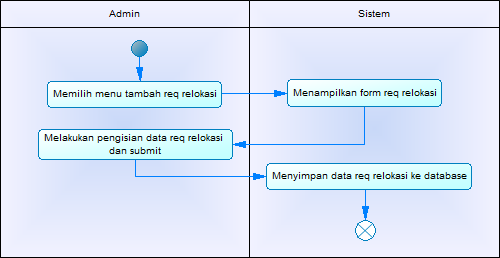
\includegraphics[width=9cm,height=6cm]{bab4/ActivityDiagram_MenambahkanReqRelokasi.png}}
	\caption{Diagram Aktivitas Menambah Request Relokasi}
	\label{figure:activity_menambah_req_relokasi}
	\end{figure}
		
	\subsubsection{Mengubah Request Relokasi}
	User dapat mengubah permintaan relokasi. Diagram \ref{figure:activity_mengubah_req_relokasi} adalah diagram aktivitas mengubah permintaan relokasi pada sistem \textit{Monitoring} SIK.
	\begin{figure}[h]
	\centerline {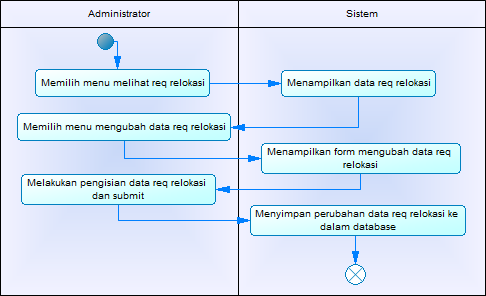
\includegraphics[width=9cm,height=5cm]{bab4/ActivityDiagram_MengubahReqRelokasi.png}}
	\caption{Diagram Aktivitas Mengubah Request Relokasi}
	\label{figure:activity_mengubah_req_relokasi}
	\end{figure}

	\subsubsection{Menghapus Request Relokasi}
	User dapat menghapus permintaan relokasi. Diagram \ref{figure:activity_menghapus_req_relokasi} adalah diagram aktivitas menghapus permintaan relokasi pada sistem \textit{Monitoring} SIK.
	\begin{figure}[h]
	\centerline {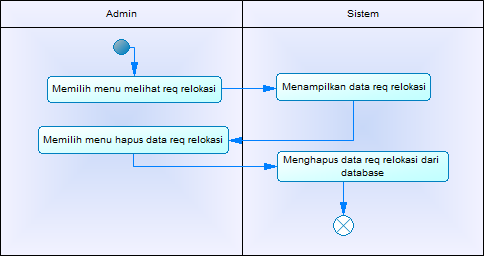
\includegraphics[width=9cm,height=5cm]{bab4/ActivityDiagram_MenghapusReqRelokasi.png}}
	\caption{Diagram Aktivitas Menghapus Request Relokasi}
	\label{figure:activity_menghapus_req_relokasi}
	\end{figure}		

	\begin{figure}[h]
	\centerline {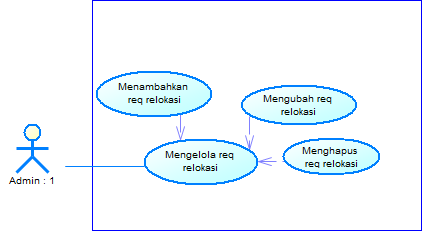
\includegraphics[width=8cm,height=4.5cm]{bab4/use-case-mengelola-req-relokasi.png}}
	\caption{Diagram \textit{Use Case} Mengelola Request Relokasi}
	\label{figure:use_case_mengelola_req_relokasi}
	\end{figure}

\section{Mengelola SIK}
Berikut adalah deskripsi dan diagram aktivitas pada \textit{use case} Mengelola SIK.
\subsection{Deskripsi Umum Sistem}
\tab Sistem ini akan melakukan pengelolaan SIK(Surat Izin Kerja). Pembuatan SIK didasarkan pada permintaan relokasi yang ada pada daftar permintaan relokasi. Daftar-daftar permintaan relokasi yang telah dibuatkan SIK tidak akan dimunculkan kembali pada saat pengisian formulir penambahan SIK. Data yang dimasukkan akan disimpan ke dalam basis data.
\subsection{\textit{Use Case} dan Fitur Sistem}
Gambar \ref{figure:use_case_mengelola_sik} adalah \textit{use case} mengelola SIK. Pada pengelolaan SIK, user dapat melakukan beberapa kegiatan sebagai berikut:
	\subsubsection{Menambah SIK}
	User dapat menambahkan SIK berdasarkan permintaan relokasi yang ada. Batasan dalam pembuatan SIK yaitu setiap SIK harus dikerjakan oleh provider yang sama. Pada saat pembuatan SIK, permintaan relokasi yang telah dibuatkan SIK tidak akan ditampilkan ulang pada daftar permintaan relokasi yang ada. Diagram \ref{figure:activity_menambah_sik} adalah diagram aktivitas menambah SIK pada sistem \textit{Monitoring} SIK.
	\begin{figure}[h]
	\centerline {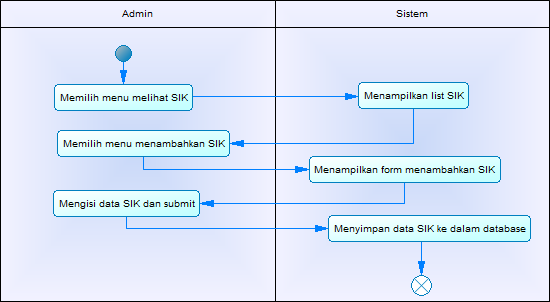
\includegraphics[width=9cm,height=6cm]{bab4/ActivityDiagram_MenambahkanSIK.png}}
	\caption{Diagram Aktivitas Menambah SIK}
	\label{figure:activity_menambah_sik}
	\end{figure}
		
	\subsubsection{Mengubah SIK}
	User dapat mengubah data SIK yang telah ditambahkan. Diagram \ref{figure:activity_mengubah_sik} adalah diagram aktivitas mengubah SIK pada sistem Monitoring SIK.
	\begin{figure}[h]
	\centerline {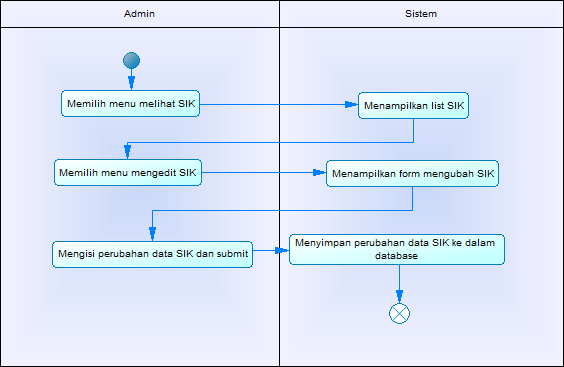
\includegraphics[width=9cm,height=5.6cm]{bab4/ActivityDiagram_MengubahSIK.png}}
	\caption{Diagram Aktivitas Mengubah SIK}
	\label{figure:activity_mengubah_sik}
	\end{figure}

	\subsubsection{Menghapus SIK}
	User dapat menghapus SIK. Pada penghapusan SIK, permintaan relokasi yang SIKnya dihapus akan ditampilkan ulang pada daftar permintaan relokasi. Diagram \ref{figure:activity_menghapus_sik} adalah diagram aktivitas menghapus SIK pada sistem \textit{Monitoring } SIK.
	\begin{figure}[h]
	\centerline {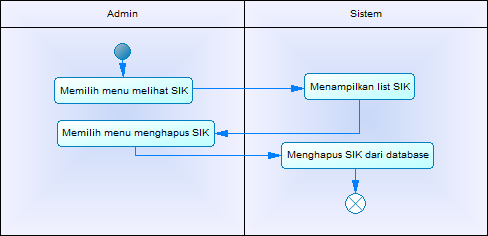
\includegraphics[width=9cm,height=4.5cm]{bab4/ActivityDiagram_MenghapusSIK.png}}
	\caption{Diagram Aktivitas Menghapus SIK}
	\label{figure:activity_menghapus_sik}
	\end{figure}		

	\begin{figure}[h]
	\centerline {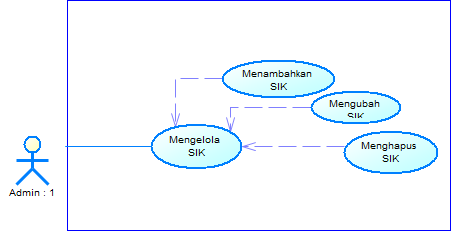
\includegraphics[width=9cm,height=5cm]{bab4/use-case-mengelola-sik.png}}
	\caption{Diagram \textit{Use Case} Mengelola SIK}
	\label{figure:use_case_mengelola_sik}
	\end{figure}

\section{Mengelola Eksekusi}
Berikut adalah deskripsi dan diagram aktivitas pada \textit{use case} Mengelola Eksekusi.
\subsection{Deskripsi Umum Sistem}
\tab Sistem ini akan melakukan pengelolaan eksekusi permintaan relokasi. Pengelolaan eksekusi permintaan relokasi didasarkan pada SIK yang telah dibuat. Apabila SIK sudah masuk tahap \textit{approval} oleh kepala divisi, selanjutkan masuk pada tahap eksekusi.
\subsection{\textit{Use Case} dan Fitur Sistem}
Gambar \ref{figure:use_case_mengelola_eksekusi} adalah \textit{use case} mengelola eksekusi permintaan relokasi. Pada pengelolaan eksekusi permintaan relokasi, user dapat melakukan beberapa kegiatan sebagai berikut:
	\subsubsection{Menambah Eksekusi}
	User dapat menambahkan eksekusi permintaan relokasi berdasarkan pada SIK yang ada. Penambahan eksekusi dilakukan dengan pengubahan status SIK dari proses menjadi \textit{approved}. Diagram \ref{figure:activity_menambah_eksekusi} adalah diagram aktivitas menambah eksekusi request relokasi pada sistem \textit{Monitoring} SIK.
	\begin{figure}[h]
	\centerline {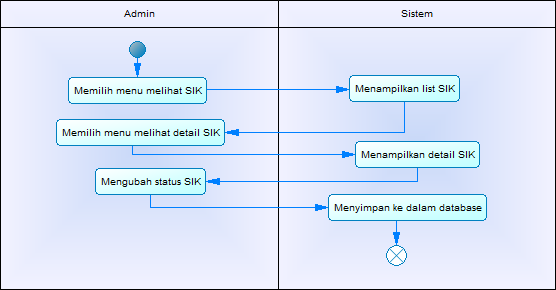
\includegraphics[width=9cm,height=6cm]{bab4/ActivityDiagram_MenambahkanEksekusi.png}}
	\caption{Diagram Aktivitas Menambah Eksekusi Request Relokasi}
	\label{figure:activity_menambah_eksekusi}
	\end{figure}
		
	\subsubsection{Mengubah Eksekusi}
	User dapat mengubah eksekusi permintaan relokasi yang telah dibuat. Perubahan pada data eksekusi akan disimpan menggantikan data yang sebelumnya telah dibuat. Diagram \ref{figure:activity_mengubah_eksekusi} adalah diagram aktivitas mengubah eksekusi permintaan relokasi pada sistem \textit{Monitoring} SIK.
	\begin{figure}[h]
	\centerline {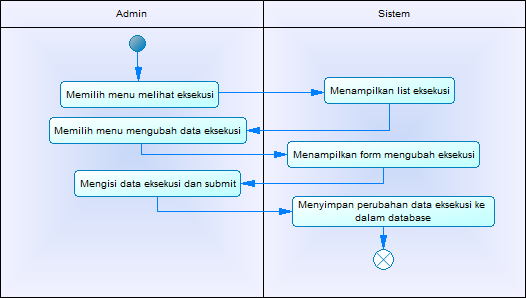
\includegraphics[width=9cm,height=4.6cm]{bab4/ActivityDiagram_MengubahEksekusi.png}}
	\caption{Diagram Aktivitas Mengubah Eksekusi Request Relokasi}
	\label{figure:activity_mengubah_eksekusi}
	\end{figure}

	\subsubsection{Menghapus Eksekusi}
	User dapat menghapus eksekusi permintaan relokasi. Dan mengembalikan status eksekusi menjadi proses pembuatan SIK. Diagram \ref{figure:activity_menghapus_eksekusi} adalah diagram aktivitas menghapus eksekusi permintaan relokasi pada sistem \textit{Monitoring} SIK.
	\begin{figure}[h]
	\centerline {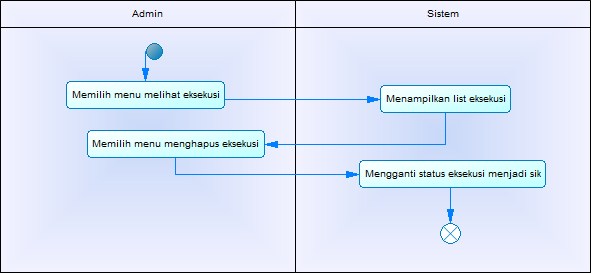
\includegraphics[width=9cm,height=4.5cm]{bab4/ActivityDiagram_MenghapusEksekusi.png}}
	\caption{Diagram Aktivitas Menghapus Eksekusi Request Relokasi}
	\label{figure:activity_menghapus_eksekusi}
	\end{figure}		

	\begin{figure}[h]
	\centerline {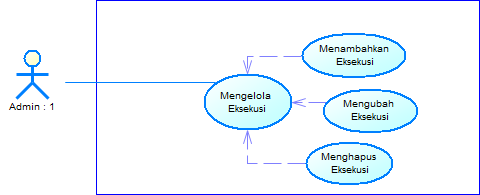
\includegraphics[width=9cm,height=5cm]{bab4/use-case-mengelola-eksekusi.png}}
	\caption{Diagram \textit{Use Case} Mengelola Eksekusi Request Relokasi}
	\label{figure:use_case_mengelola_eksekusi}
	\end{figure}

\section{Mengelola Penagihan}
Berikut adalah deskripsi dan diagram aktivitas pada \textit{use case} Mengelola Penagihan.
\subsection{Deskripsi Umum Sistem}
\tab Sistem ini akan melakukan pengelolaan penagihan permintaan relokasi. Pengelolaan penagihan permintaan relokasi didasarkan pada proses sebelumnya. Setelah proses eksekusi selesai, status SIK akan diubah menjadi penagihan pembayaran.
\subsection{\textit{Use Case} dan Fitur Sistem}
Gambar \ref{figure:use_case_mengelola_penagihan} adalah \textit{use case} mengelola penagihan permintaan relokasi. Pada pengelolaan penagihan permintaan relokasi, user dapat melakukan beberapa kegiatan sebagai berikut:
	\subsubsection{Menambah Penagihan}
	User dapat menambahkan penagihan permintaan relokasi. Berdasarkan pada proses sebelumnya, yaitu eksekusi. Penambahan proses penagihan dilakukan dengan pengubahan status SIK dari eksekusi menjadi penagihan. Diagram \ref{figure:activity_menambah_penagihan} adalah diagram aktivitas menambah penagihan permintaan relokasi pada sistem \textit{Monitoring} SIK.
	\begin{figure}[h]
	\centerline {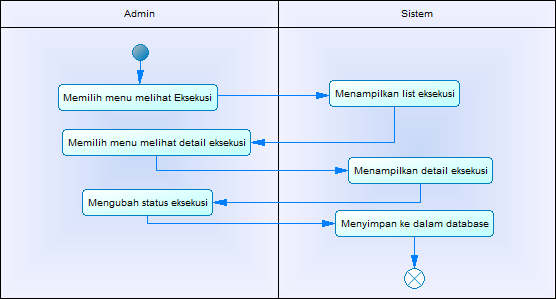
\includegraphics[width=9cm,height=4.6cm]{bab4/ActivityDiagram_MenambahkanPenagihan.png}}
	\caption{Diagram Aktivitas Menambah Penagihan Request Relokasi}
	\label{figure:activity_menambah_penagihan}
	\end{figure}
	\subsubsection{Mengubah Penagihan}
	User dapat mengubah penagihan permintaan relokasi yang telah dibuat. Perubahan penagihan yang dibuat akan menggantikan data yang sebelumnya dibuat. Diagram \ref{figure:activity_mengubah_penagihan} adalah diagram aktivitas mengubah penagihan permintaan relokasi pada sistem Monitoring SIK.
	\begin{figure}[h]
	\centerline {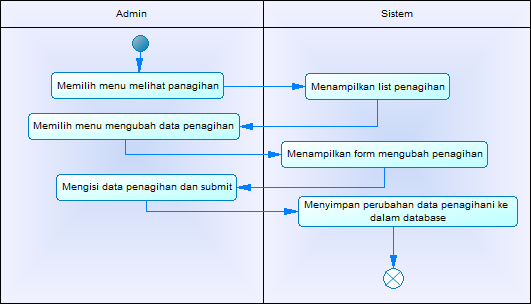
\includegraphics[width=9cm,height=6cm]{bab4/ActivityDiagram_MengubahPenagihan.png}}
	\caption{Diagram Aktivitas Mengubah Penagihan Request Relokasi}
	\label{figure:activity_mengubah_penagihan}
	\end{figure}
	
	\subsubsection{Menghapus Penagihan}
	User dapat menghapus penagihan permintaan relokasi. proses penghapusan data penagihan akan mengembalikan proses penagihan menjadi proses eksekusi. Diagram \ref{figure:activity_menghapus_penagihan} adalah diagram aktivitas menghapus penagihan permintaan relokasi pada sistem \textit{Monitoring} SIK.
	\begin{figure}[h]
	\centerline {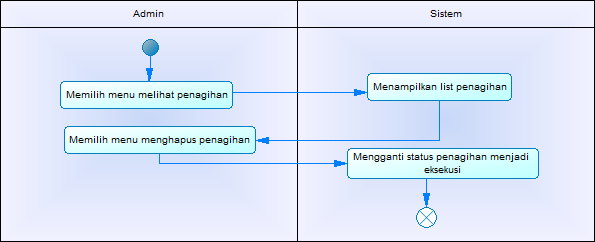
\includegraphics[width=9cm,height=4cm]{bab4/ActivityDiagram_MenghapusPenagihan.png}}
	\caption{Diagram Aktivitas Menghapus Penagihan Request Relokasi}
	\label{figure:activity_menghapus_penagihan}
	\end{figure}		

	\begin{figure}[h]
	\centerline {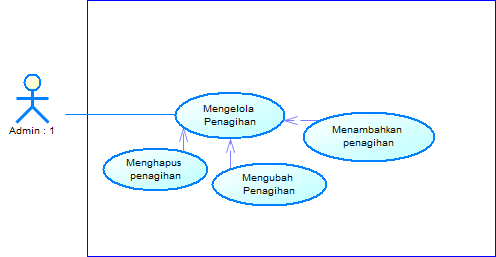
\includegraphics[width=9cm,height=5cm]{bab4/use-case-mengelola-penagihan.png}}
	\caption{Diagram \textit{Use Case} Mengelola Penagihan Request Relokasi}
	\label{figure:use_case_mengelola_penagihan}
	\end{figure}

\section{Melihat Request Relokasi}
Berikut adalah deskripsi dan diagram aktivitas pada \textit{use case} Melihat Request Relokasi.
\subsection{Deskripsi Umum Sistem}
\tab Sistem dapat menampilkan daftar permintaan relokasi kepada user berdasarkan \textit{record} yang tersimpan dalam basis data.
\subsection{\textit{Use Case} dan Fitur Sistem}
Gambar \ref{figure:use_case_melihat_req_relokasi} adalah \textit{use case} melihat daftar permintaan relokasi. Pada halaman melihat permintaan relokasi, user dapat melakukan beberapa kegiatan sebagai berikut:
	\subsubsection{Melihat Request Relokasi}
	User dapat melihat daftar permintaan relokasi yang telah ditambahkan ke dalam basis data. Diagram \ref{figure:activity_melihat_req_relokasi} adalah diagram aktivitas melihat daftar permintaan relokasi pada sistem \textit{Monitoring} SIK.
	\begin{figure}[h]
	\centerline {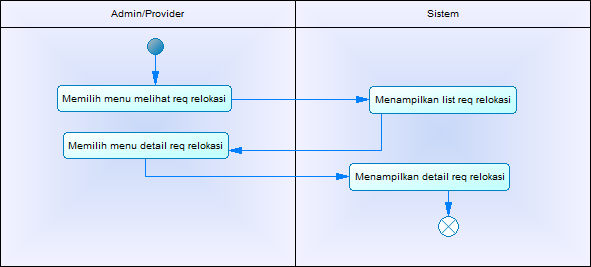
\includegraphics[width=9cm,height=4.5cm]{bab4/ActivityDiagram_MelihatReqRelokasi.png}}
	\caption{Diagram Aktivitas Melihat Daftar Request Relokasi}
	\label{figure:activity_melihat_req_relokasi}
	\end{figure}
	
	\subsubsection{Men\textit{download} Request Relokasi}
	User dapat men\textit{download} surat permintaan relokasi yang telah di\textit{upload} ke dalam basis data. Diagram \ref{figure:activity_mendownload_req_relokasi} adalah aktivitas diagram men\textit{download} surat permintaan relokasi pada sistem \textit{Monitoring} SIK.
	\begin{figure}[h]
	\centerline
	{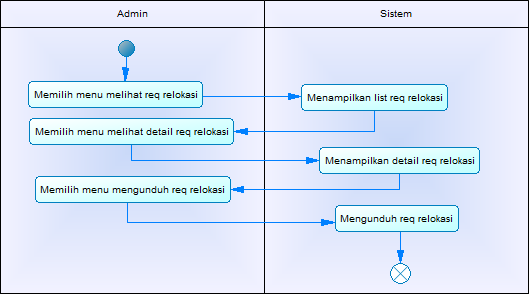
\includegraphics[width=9cm,height=5cm]{bab4/ActivityDiagram_DownloadReqRelokasi.png}}
	\caption{Diagram Aktivitas Mendownload Request Relokasi}
	\label{figure:activity_mendownload_req_relokasi}
	\end{figure}

	\begin{figure}[h]
	\centerline
	{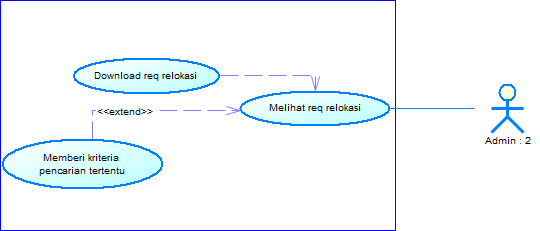
\includegraphics[width=9cm,height=5cm]{bab4/use-case-melihat-req-relokasi.png}}
	\caption{Diagram \textit{Use Case} Melihat Request Relokasi}
	\label{figure:use_case_melihat_req_relokasi}
	\end{figure}

\section{Melihat SIK}
Berikut adalah deskripsi dan diagram aktivitas pada \textit{use case} Melihat SIK.
\subsection{Deskripsi Umum Sistem}
\tab Sistem dapat menampilkan daftar SIK kepada user berdasarkan \textit{record} yang tersimpan dalam basis data.
\subsection{\textit{Use Case} dan Fitur Sistem}
Gambar \ref{figure:use_case_melihat_sik} adalah \textit{use case} melihat daftar SIK. Pada halaman melihat daftar SIK, user dapat melakukan beberapa kegiatan sebagai berikut:
	\subsubsection{Melihat SIK}
	User dapat melihat daftar SIK yang telah ditambahkan ke dalam basis data. Diagram \ref{figure:activity_melihat_sik} adalah diagram aktivitas melihat daftar SIK pada sistem \textit{Monitoring} SIK.
	\begin{figure}[h]
	\centerline {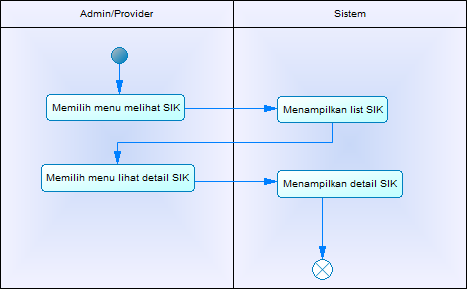
\includegraphics[width=9cm,height=5cm]{bab4/ActivityDiagram_MelihatSIK.png}}
	\caption{Diagram Aktivitas Melihat Daftar SIK}
	\label{figure:activity_melihat_sik}
	\end{figure}
	
	\subsubsection{Men\textit{download} SIK}
	User dapat men\textit{download} SIK yang telah di\textit{upload} ke dalam basis data. Diagram \ref{figure:activity_mendownload_sik} adalah aktivitas diagram men\textit{download} SIK pada sistem \textit{Monitoring} SIK.
	\begin{figure}[h]
	\centerline
	{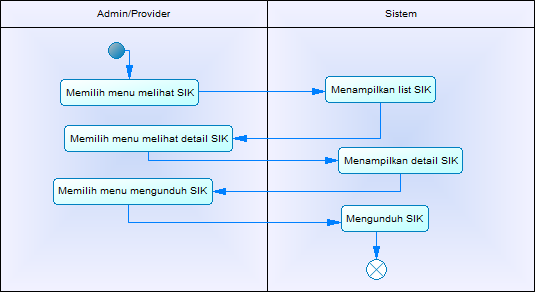
\includegraphics[width=9cm,height=5cm]{bab4/ActivityDiagram_DownloadSIK.png}}
	\caption{Diagram Aktivitas Mendownload SIK}
	\label{figure:activity_mendownload_sik}
	\end{figure}

	\begin{figure}[h]
	\centerline
	{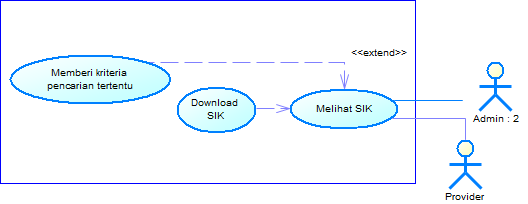
\includegraphics[width=9cm,height=5cm]{bab4/use-case-melihat-sik.png}}
	\caption{Diagram \textit{Use Case} Melihat SIK}
	\label{figure:use_case_melihat_sik}
	\end{figure}
	
\section{Melihat Eksekusi}
Berikut adalah deskripsi dan diagram aktivitas pada \textit{use case} Melihat Eksekusi.
\subsection{Deskripsi Umum Sistem}
\tab Sistem dapat menampilkan daftar eksekusi permintaan relokasi. Daftar eksekusi permintaan relokasi ditampilkan berdasarkan SIK yang memiliki status \textit{approval}.
\subsection{\textit{Use Case} dan Fitur Sistem}
Gambar \ref{figure:use_case_melihat_eksekusi} adalah \textit{use case} melihat daftar eksekusi permintaan relokasi. Pada halaman melihat daftar eksekusi permintaan relokasi, user dapat melakukan beberapa kegiatan sebagai berikut:
	\subsubsection{Melihat Ekekusi}
	User dapat melihat daftar eksekusi permintaan relokasi berdasarkan daftar SIK dengan status \textit{approval}. Diagram \ref{figure:activity_melihat_eksekusi} adalah diagram aktivitas melihat daftar eksekusi permintaan relokasi pada sistem \textit{Monitoring} SIK.
	\begin{figure}[h]
	\centerline {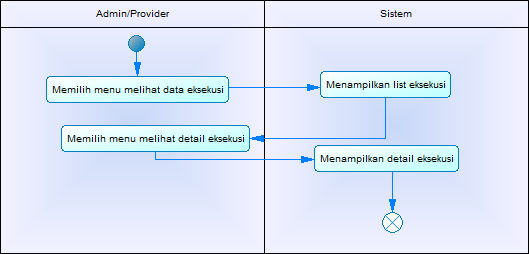
\includegraphics[width=9cm,height=4.6cm]{bab4/ActivityDiagram_MelihatEksekusi.png}}
	\caption{Diagram Aktivitas Melihat Daftar Eksekusi}
	\label{figure:activity_melihat_eksekusi}
	\end{figure}
	
	\subsubsection{Men\textit{download} Berita Acara}
	User dapat men\textit{download} berita acara yang telah di\textit{upload} ke dalam basis data. Diagram \ref{figure:activity_mendownload_berita_acara} adalah aktivitas diagram men\textit{download} berita acara pada sistem \textit{Monitoring} SIK.
	\begin{figure}[h]
	\centerline
	{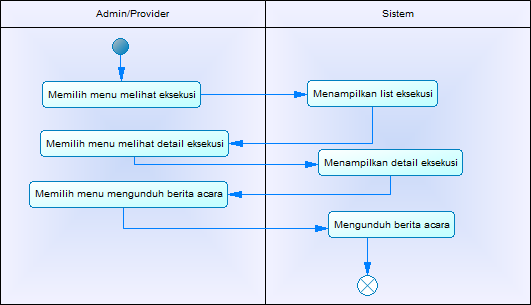
\includegraphics[width=9cm,height=4.6cm]{bab4/ActivityDiagram_DownloadBeritaAcara.png}}
	\caption{Diagram Aktivitas Mendownload Berita Acara}
	\label{figure:activity_mendownload_berita_acara}
	\end{figure}
	
	\subsubsection{Men\textit{download} Tagihan}
	User dapat men\textit{download} penagihan pembayaran yang telah di\textit{upload} ke dalam basis data. Diagram \ref{figure:activity_mendownload_tagihan} adalah aktivitas diagram men\textit{download} penagihan pembayaran pada sistem \textit{Monitoring} SIK.
	\begin{figure}[h]
	\centerline
	{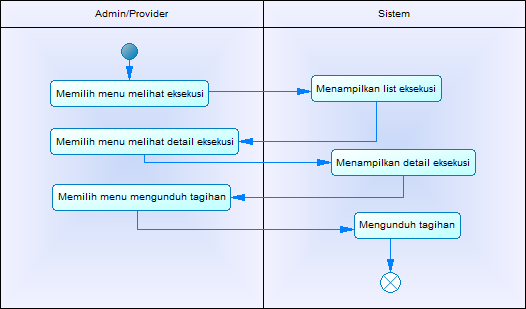
\includegraphics[width=9cm,height=5cm]{bab4/ActivityDiagram_DownloadTagihan.png}}
	\caption{Diagram Aktivitas Mendownload Tagihan Pembayaran}
	\label{figure:activity_mendownload_tagihan}
	\end{figure}

	\begin{figure}[h!]
	\centerline
	{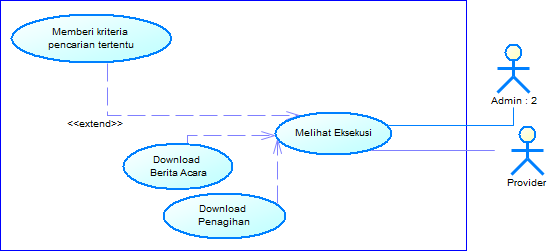
\includegraphics[width=9cm,height=5cm]{bab4/use-case-melihat-eksekusi.png}}
	\caption{Diagram \textit{Use Case} Melihat Eksekusi}
	\label{figure:use_case_melihat_eksekusi}
	\end{figure}
	
\section{Melihat Penagihan}
Berikut adalah deskripsi dan diagram aktivitas pada \textit{use case} Melihat Penagihan.
\subsection{Deskripsi Umum Sistem}
\tab Sistem dapat menampilkan daftar penagihan pembayaran permintaan relokasi. Daftar penagihan pembayaran permintaan relokasi didasarkan pada proses eksekusi yang memiliki status \textit{finish}. Pada halaman ini, user dapat melihat proses-proses penagihan pembayaran dari kegiatan-kegiatan relokasi yang dikerjakan.
\subsection{\textit{Use Case} dan Fitur Sistem}
Gambar \ref{figure:use_case_melihat_penagihan} adalah \textit{use case} melihat daftar penagihan pembayaran permintaan relokasi. Pada halaman melihat daftar penagihan pembayaran permintaan relokasi, user dapat melakukan beberapa kegiatan sebagai berikut:
	\subsubsection{Melihat Penagihan}
	User dapat melihat daftar penagihan pembayaran permintaan relokasi berdasarkan daftar proses eksekusi dengan status \textit{finish}. Diagram \ref{figure:activity_melihat_penagihan} adalah diagram aktivitas melihat daftar penagihan pembayaran permintaan relokasi pada sistem \textit{Monitoring} SIK.
	
	\begin{figure}[h!]
	\centerline {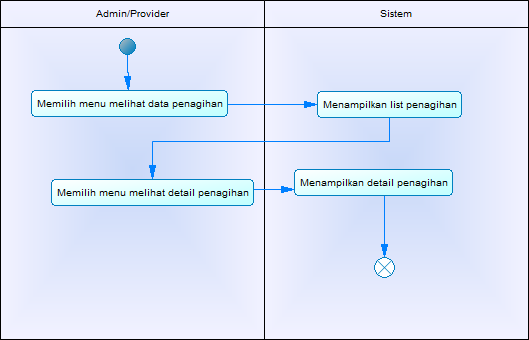
\includegraphics[width=9cm,height=5cm]{bab4/ActivityDiagram_MelihatPenagihan.png}}
	\caption{Diagram Aktivitas Melihat Daftar Penagihan Pembayaran}
	\label{figure:activity_melihat_penagihan}
	\end{figure}

	\begin{figure}[h!]
	\centerline
	{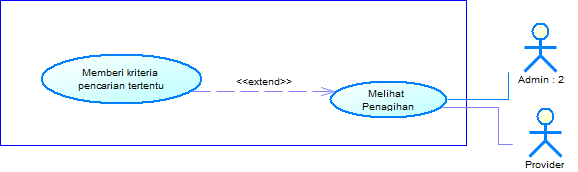
\includegraphics[width=9cm,height=5.5cm]{bab4/use-case-melihat-penagihan.png}}
	\caption{Diagram \textit{Use Case} Melihat Penagihan Pembayaran}
	\label{figure:use_case_melihat_penagihan}
	\end{figure}
	
\section{Melihat Finish}
Berikut adalah deskripsi dan diagram aktivitas pada \textit{use case} Melihat Finish.
\subsection{Deskripsi Umum Sistem}
\tab Sistem dapat menampilkan daftar permintaan relokasi dengan status telah dibayar.
\subsection{\textit{Use Case} dan Fitur Sistem}
Gambar \ref{figure:use_case_melihat_finish} adalah \textit{use case} melihat daftar permintaan relokasi dengan status telah dibayar. Pada halaman melihat daftar permintaan relokasi dengan status telah dibayar, user dapat melakukan beberapa kegiatan sebagai berikut:
	\subsubsection{Melihat Finish}
	User dapat melihat daftar permintaan relokasi dengan status telah dibayar. Diagram \ref{figure:activity_melihat_finish} adalah diagram aktivitas melihat daftar penagihan pembayaran permintaan relokasi pada sistem \textit{Monitoring} SIK.
	\begin{figure}[h]
	\centerline {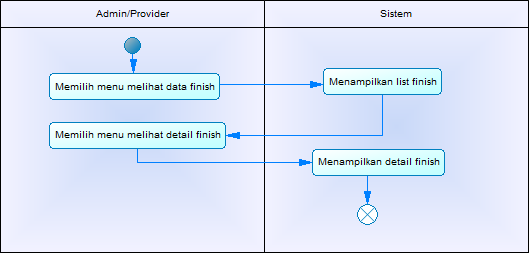
\includegraphics[width=9cm,height=5.5cm]{bab4/ActivityDiagram_MelihatFinish.png}}
	\caption{Diagram Aktivitas Melihat Daftar Permintaan Relokasi Sudah Dibayar}
	\label{figure:activity_melihat_finish}
	\end{figure}

	\begin{figure}[h!]
	\centerline
	{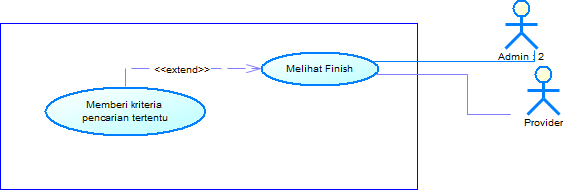
\includegraphics[width=9cm,height=5cm]{bab4/use-case-melihat-finish.png}}
	\caption{Diagram \textit{Use Case} Melihat Daftar Permintaan Relokasi Sudah Dibayar}
	\label{figure:use_case_melihat_finish}
	\end{figure}
	
\newpage
\section{Perancangan Data}
\tab Dalam pembuatan sebuah sistem informasi, database merupakan salah satu faktor utama yang penting. Perancangan dan alur data pada sebuah sistem harus dapat memenuhi kebutuhan-kebutuhan sistem, meliputi penambahan data, perubahan isi data dan penghapusan data dari basisdata sistem. Berikut adalah perancangan data pada sistem informasi \textit{monitoring} SIK.
\subsection{\textit{Conceptual Data Model}}
CDM (\textit{Conceptual Data Model}) merupakan sebuah model yang didasarkan pada objek-objek di dunia nyata. Objek dasar tersebut direpresentasikan dalam bentuk \textit{entity relationship diagram}. Gambar \ref{figure:CDM} adalah CDM pada pembuatan sistem informasi \textit{monitoring} SIK.
	\begin{figure}[h!]
	\centerline
	{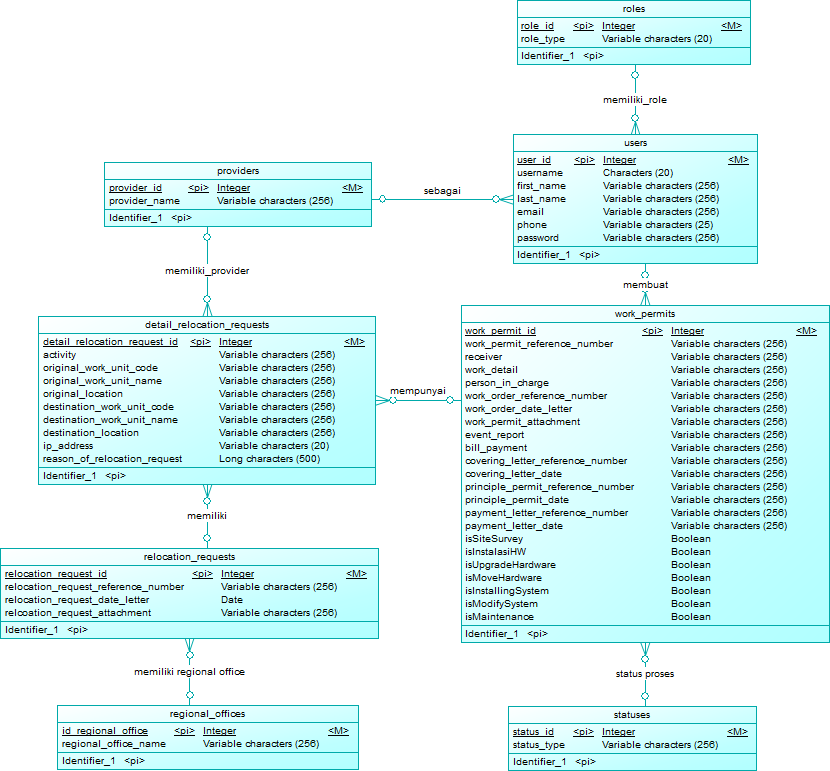
\includegraphics[width=10cm,height=14cm]{bab4/CDM.png}}
	\caption{Diagram \textit{Conceptual Data Model}}
	\label{figure:CDM}
	\end{figure}
	
\subsection{\textit{Physical Data Model}}
PDM (\textit{Physical Data Model}) adalah model yang digambarkan dalam sebuah tabel serta hubungan-hubungan antara data dengan tabel lain. Gambar \ref{figure:PDM} adalah PDM pada pembuatan sistem informasi \textit{monitoring} SIK.
	\begin{figure}[h!]
	\centerline
	{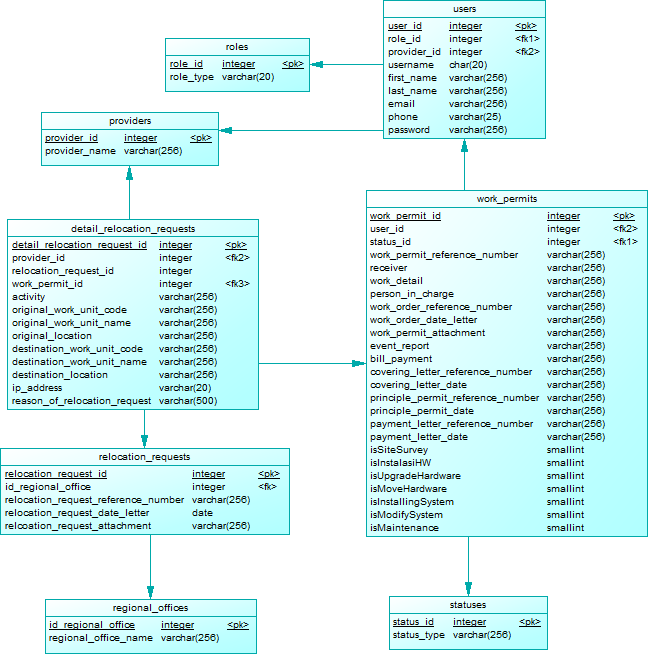
\includegraphics[width=10cm,height=11cm]{bab4/PDM.png}}
	\caption{Diagram \textit{Physical Data Model}}
	\label{figure:PDM}
	\end{figure}
	\chapter{IMPLEMENTASI}
\tab Pada bab ini akan dipaparkan implementasi dari sistem yang telah dibangun. Bahasa pemrograman yang digunakan adalah bahasa pemrograman Arduino (\textit{Sketch}) yang menyerupai bahasa C untuk memprogram mikrokontroler dan Python untuk menghubungkan mikrokontroler dengan Bot Telegram sebagai pengendali mikrokontrolernya.

\section{Lingkungan Implementasi}
\tab Lingkungan implementasi dalam pembuatan sistem "EasyMeeting" meliputi perangkat keras dan perangkat lunak yang digunakan untuk mengimplementasikan sistem yang telah dirancang adalah sebagai berikut:
\begin{enumerate}
	\item Perangkat Keras
	\begin{itemize}
		\item Komponen Mikrokontroler
		\begin{itemize}
			\item NodeMCU
			\item DHT11
			\item \textit{Breadboard}
			\item Resistor
			\item \textit{Jumper Wires}
			\item LED \textit{Light Bulb}
			\item \textit{Infrared Sensor Module}
			\item \textit{Infrared Receiver Module}
		\end{itemize}
		\item Laptop
		\begin{itemize}
			\item \textit{Processor} Intel(R) Core(TM) i7-4510U CPU @ 2.00GHz
			\item Memori 4 GB (3,92514 GB)
		\end{itemize}
	\end{itemize}
	\item Perangkat Lunak
	\begin{itemize}
		\item Sistem Operasi Linux (Linux Mint 18.3 Sylvia)
		 64-bit
		\item \textit{Text Editor} Visual Studio Code
		\item Arduino \textit{Software} IDE
		\item Bahasa Pemrograman Python
		\item \textit{Version Control System} Git
	\end{itemize}
\end{enumerate}

\section{Implementasi Rangkaian Mikrokontroler}
\tab Pada bagian ini akan dijelaskan mengenai implementasi rangkaian mikrokontroler pada sistem EasyMeeting. Untuk pengimplementasiannya, dibutuhkan beberapa komponen mikrokontroler yaitu:
\begin{itemize}
	\item NodeMCU
	\item DHT11
	\item \textit{Breadboard}
	\item Resistor
	\item \textit{Jumper Wires}
	\item LED \textit{Light Bulb}
	\item \textit{Infrared Sensor Module}
	\item \textit{Infrared Receiver Module}
\end{itemize}
\tab Semua komponen di atas kemudian dirangkai menjadi satu kesatuan sesuai dengan perancangan sistem. Langkah-langkah yang dilakukan adalah:
\begin{enumerate}
	\item Menghubungka
\end{enumerate}

\section{Implementasi Lapisan Kontrol Sistem}
\tab Pada bagian ini akan dijelaskan mengenai lapisan kontrol sistem yang berfungsi untuk mengontrol keseluruhan sistem EasyMeeting, meliputi kontrol mikrokontroler hingga menghubungkan mikrokontroler dengan antarmuka pengguna (Bot API Telegram). Lapisan kontrol sistem dibuat menggunakan bahasa pemrograman Python.

\section{Implementasi Antarmuka Pengguna}
\tab Pada bagian ini akan dijelaskan mengenai bagaimana pengguna dapat berinteraksi dengan sistem EasyMeeting melalui platform Telegram. Telegram menyediakan dua jenis API yang dapat dikembangkan bebas oleh pengguna, yakni Telegram API dan Bot API. Penulis memanfaatkan Bot API Telegram untuk membuat antarmuka sistem berupa \textit{chat bot} yang dapat berinteraksi dengan pengguna.
\tab Langkah-langkah yang dilakukan untuk membuat

\subsection{Menyalakan Lampu dan AC Ruangan}

\subsection{Mematikan Lampu dan AC Ruangan}

\subsection{Melihat Status Kondisi Lampu dan AC Ruangan}

\subsection{Mengukur Suhu Ruangan}


\subsection{Tampilan Halaman Menambahkan \textit{Request} Relokasi}
Pada halaman menambahkan \textit{request} relokasi menggunakan HTML, CSS, PHP dan Javascript. Sebuah \textit{form} ditampilkan kemudian user mengisikan data-data yang diperlukan. \textit{Form} tersebut akan menampung data-data yang diperlukan, kemudian akan disimpan ke dalam basis data sistem. Gambar \ref{figure:tambahReqRelokasi} adalah tampilan dan gambar \ref{lst:addrelokasi1}, \ref{lst:addrelokasi2} dan \ref{lst:addrelokasi3} adalah potongan kode halaman menambahkan \textit{request} relokasi.
\begin{figure}[h!]
\centerline
{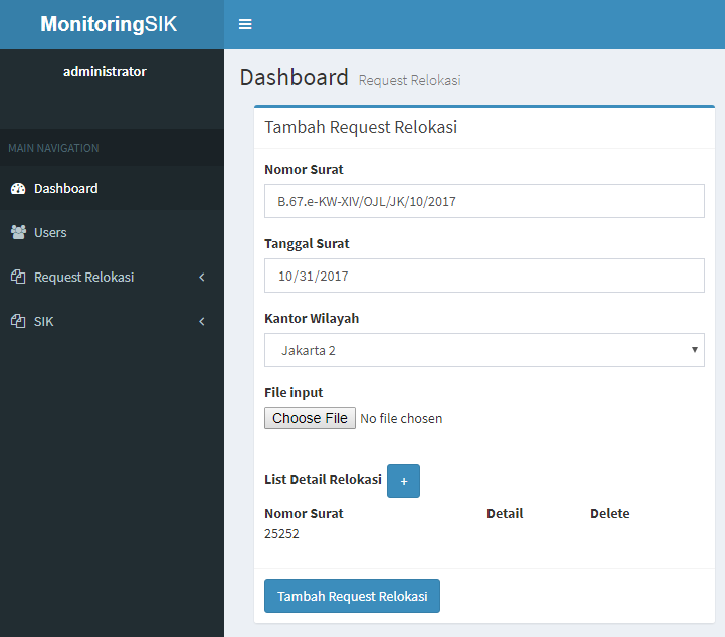
\includegraphics[width=10cm,height=7.5cm]{bab5/addReqRelokasi.png}}
\caption{Potongan Halaman Menambahkan \textit{Request} Relokasi}
\label{figure:tambahReqRelokasi}
\end{figure}

\lstinputlisting[language=PHP, firstline=34, lastline=45, firstnumber=1, caption=Potongan Kode Tampilan Menambahkan \textit{Request} Relokasi (1), label={lst:addrelokasi1}]{bab5/src/RelocationRequestController.php}
\lstinputlisting[language=PHP, firstline=46, lastline=82, firstnumber=14, caption=Potongan Kode Tampilan Menambahkan \textit{Request} Relokasi (2), label={lst:addrelokasi2}]{bab5/src/RelocationRequestController.php}
\lstinputlisting[language=PHP, firstline=83, lastline=109, firstnumber=51, caption=Potongan Kode Tampilan Menambahkan \textit{Request} Relokasi (3), label={lst:addrelokasi3}]{bab5/src/RelocationRequestController.php}


	\chapter{HASIL DAN UJI COBA}
\tab Pada bab ini akan dipaparkan hasil uji coba saat sistem dijalankan. Uji coba sistem \textit{Monitoring} SIK akan dilakukan untuk memastikan kualitas perangkat lunak yang dikembangkan dengan analisis dan perancangan perangkat lunak.

\section{Lingkungan Uji Coba}
Lingkungan uji coba sistem pada Kerja Praktik kali ini meliputi perangkat keras dan perangkat lunak adalah sebagai berikut:
\begin{enumerate}
\item Perangkat Keras
	\begin{enumerate}
	\item \textit{Processor} Intel(R) Core i3-330M @ 2.13 GHz
	\item Memori 4GB
	\end{enumerate}
\item Perangkat Lunak
	\begin{enumerate}
	\item Sistem Operasi Windows 10 64 bit
	\end{enumerate}
\end{enumerate}

\section{Skenario Pengujian}
Skenario pengujian yang akan dilakukan pada aplikasi \textit{Monitoring} SIK adalah melakukan peran sebagai admin yang sedang membuka aplikasi. Langkah-langkah dari skenario adalah sebagai berikut:
	\begin{enumerate}
	\item User membuka aplikasi \textit{Monitoring} SIK.
	\item User memilih menu \textit{request} relokasi, SIK, eksekusi, penagihan dan finish.
	\item User menambahkan data \textit{request} relokasi dan SIK dengan mengisi \textit{form}.
	\item User melihat detail \textit{request} relokasi, SIK, eksekusi, penagihan dan finish.
	\end{enumerate}
\subsection{Pengujian Menampilkan Data \textit{Request} Relokasi}
Pengujian ini dilakukan terhadap fungsionalitas menampilkan data \textit{request} relokasi. Tabel \ref{tab:list_req_relokasi} menjelaskan pengujian fungsionalitas ini. Gambar \ref{figure:data_req_relokasi} adalah hasil fungsionalitas menampilkan data \textit{request} relokasi.

\begin{table}[h!]
	\centering
	\begin{tabular}{|p{4cm}|p{6cm}|}
	\hline
	Kode \textit{Use Case} & UC-001\\ \hline
	Tujuan Pengujian & Menampilkan semua data \textit{request} relokasi\\ \hline
	Data Masukan & - \\ \hline
	Prosedur Pengujian & 
		\begin{enumerate}
		\item Pengguna \textit{login} sebagai administrator
		\item Pengguna memilih menu \textit{request} relokasi
		\end{enumerate}\\ \hline
	Hasil yang diharapkan & Semua data \textit{request} relokasi dapat ditampilkan pada menu \textit{request} relokasi dan dapat dipilih untuk melihat detailnya \\ \hline
	Hasil yang diperoleh & Semua data \textit{request} relokasi dapat ditampilkan pada menu \textit{request} relokasi dan detailnya dapat ditampilkan\\ \hline
	Kesimpulan & Proses menampilkan data \textit{request} relokasi beserta detailnya berhasil\\ \hline
	Kondisi Akhir & Pengguna mendapatkan semua informasi data \textit{request} relokasi\\ \hline
	\end{tabular}\caption{Skenario Pengujian Menampilkan Data \textit{Request} Relokasi}
	\label{tab:list_req_relokasi}
\end{table}

\begin{figure}[h!]
\centerline
{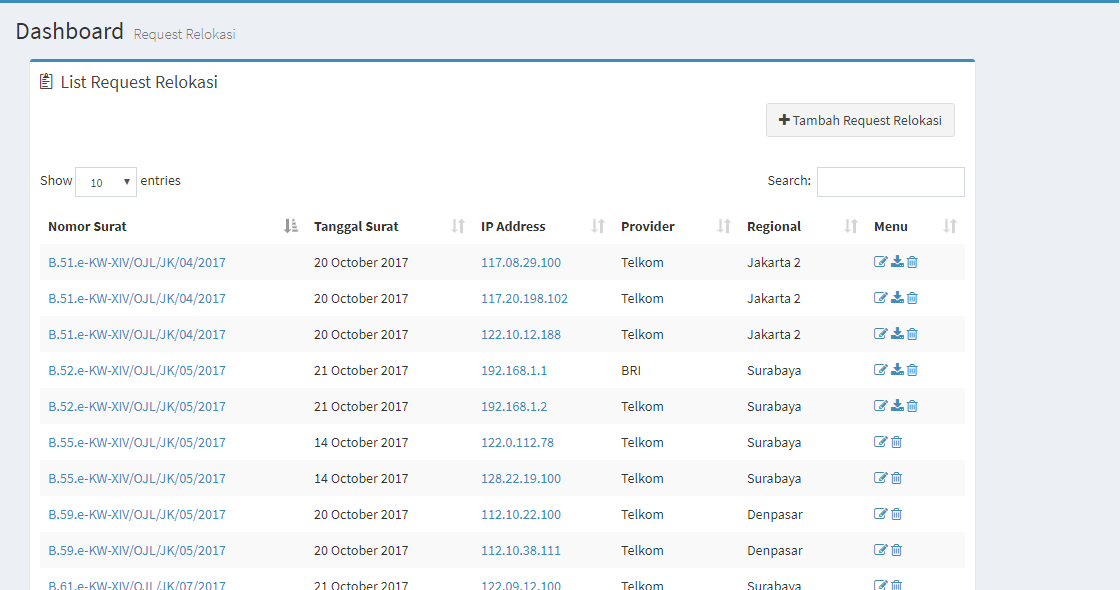
\includegraphics[width=10cm,height=5cm]{bab6/listReqRelokasi.png}}
\caption{Data \textit{Request} Relokasi}
\label{figure:data_req_relokasi}
\end{figure}

\subsection{Pengujian Menampilkan Data SIK}
Pengujian ini dilakukan terhadap fungsionalitas menampilkan data SIK. Tabel \ref{tab:list_sik} menjelaskan pengujian fungsionalitas ini. Gambar \ref{figure:data_detail_sik} adalah hasil fungsionalitas menampilkan data SIK.
\begin{figure}[h!]
\centerline
{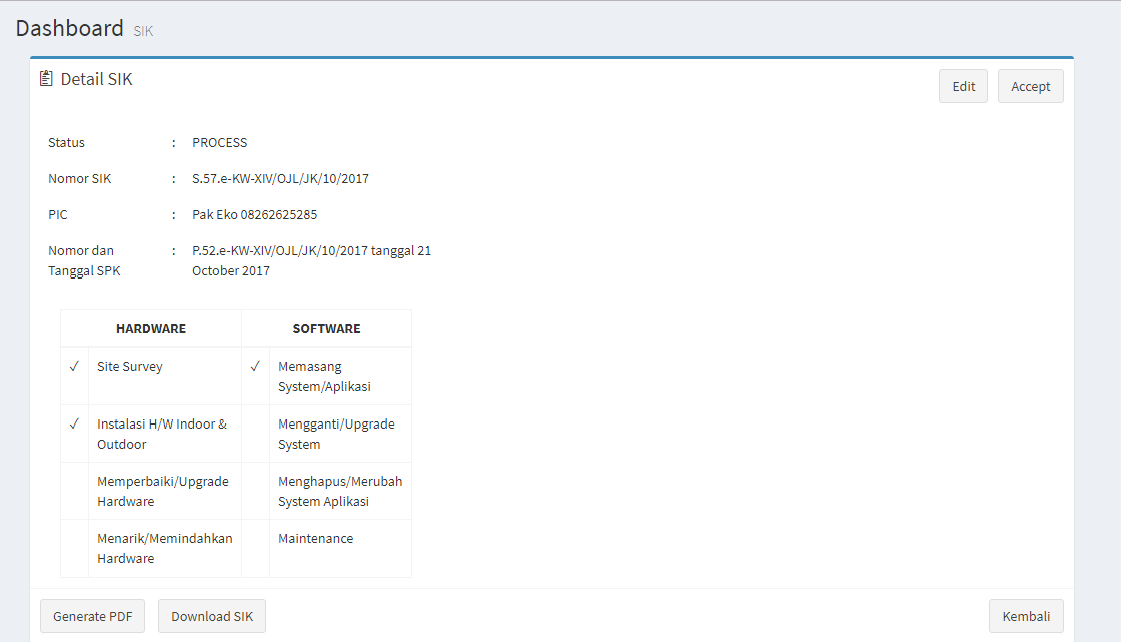
\includegraphics[width=10cm,height=5cm]{bab6/detailSIK.png}}
\caption{Data Detail SIK}
\label{figure:data_detail_sik}
\end{figure}

\begin{table}[h!]
	\centering
	\begin{tabular}{|p{4cm}|p{6cm}|}
	\hline
	Kode \textit{Use Case} & UC-002\\ \hline
	Tujuan Pengujian & Menampilkan semua data SIK\\ \hline
	Data Masukan & - \\ \hline
	Prosedur Pengujian & 
		\begin{enumerate}
		\item Pengguna \textit{login} sebagai administrator
		\item Pengguna memilih menu SIK
		\end{enumerate}\\ \hline
	Hasil yang diharapkan & Semua data SIK dapat ditampilkan pada menu SIK dan dapat dipilih untuk melihat detailnya \\ \hline
	Hasil yang diperoleh & Semua data SIK dapat ditampilkan pada menu SIK dan detailnya dapat ditampilkan\\ \hline
	Kesimpulan & Proses menampilkan data SIK beserta detailnya berhasil\\ \hline
	Kondisi Akhir & Pengguna mendapatkan semua informasi data SIK\\ \hline
	\end{tabular}\caption{Skenario Pengujian Menampilkan Data SIK}
	\label{tab:list_sik}
\end{table}

\subsection{Pengujian Menampilkan Data Eksekusi}
Pengujian ini dilakukan terhadap fungsionalitas menampilkan data Eksekusi. Tabel \ref{tab:list_eksekusi_1} dan \ref{tab:list_eksekusi_2} menjelaskan pengujian fungsionalitas ini. Gambar \ref{figure:data_detail_eksekusi} adalah hasil fungsionalitas menampilkan data Eksekusi.

\begin{table}[h!]
	\centering
	\begin{tabular}{|p{4cm}|p{6cm}|}
	\hline
	Kode \textit{Use Case} & UC-003\\ \hline
	Tujuan Pengujian & Menampilkan semua data Eksekusi\\ \hline
	Data Masukan & - \\ \hline
	\end{tabular}\caption{Skenario Pengujian Menampilkan Data Eksekusi(1)}
	\label{tab:list_eksekusi_1}
\end{table}

\begin{table}[h!]
	\centering
	\begin{tabular}{|p{4cm}|p{6cm}|}
	\hline
	Prosedur Pengujian & 
		\begin{enumerate}
		\item Pengguna \textit{login} sebagai administrator
		\item Pengguna memilih menu Eksekusi
		\end{enumerate}\\ \hline
	Hasil yang diharapkan & Semua data Eksekusi dapat ditampilkan pada menu Eksekusi dan dapat dipilih untuk melihat detailnya \\ \hline
	Hasil yang diperoleh & Semua data Eksekusi dapat ditampilkan pada menu Eksekusi dan detailnya dapat ditampilkan\\ \hline
	Kesimpulan & Proses menampilkan data Eksekusi beserta detailnya berhasil\\ \hline
	Kondisi Akhir & Pengguna mendapatkan semua informasi data Eksekusi\\ \hline
	\end{tabular}\caption{Skenario Pengujian Menampilkan Data Eksekusi(2)}
		\label{tab:list_eksekusi_2}
\end{table}

\begin{figure}[h!]
\centerline
{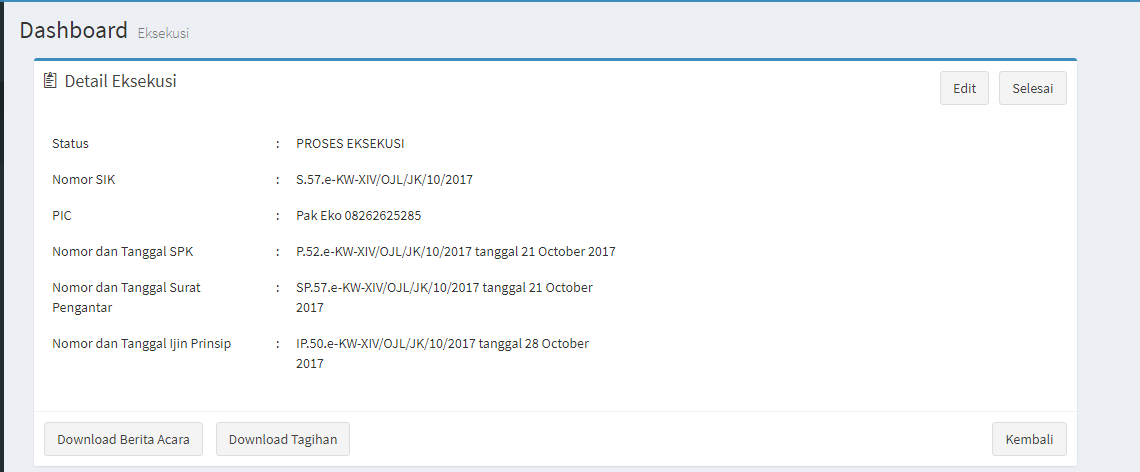
\includegraphics[width=10cm,height=5cm]{bab6/detailExecution.png}}
\caption{Data Detail Eksekusi}
\label{figure:data_detail_eksekusi}
\end{figure}

\subsection{Pengujian Menampilkan Data Penagihan}
Pengujian ini dilakukan terhadap fungsionalitas menampilkan data Penagihan. Tabel \ref{tab:list_penagihan_1} dan \ref{tab:list_penagihan_2} menjelaskan pengujian fungsionalitas ini. Gambar \ref{figure:data_detail_penagihan} adalah hasil fungsionalitas menampilkan data penagihan.
\begin{figure}[h!]
\centerline
{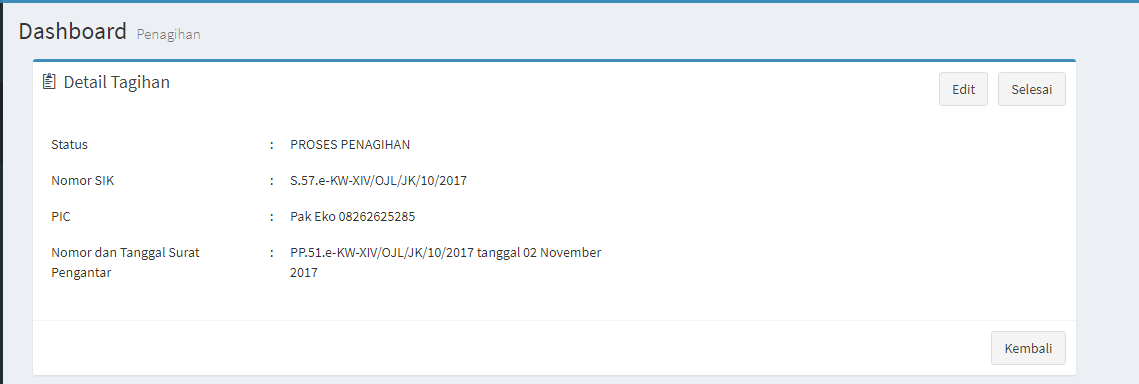
\includegraphics[width=10cm,height=4.5cm]{bab6/detailPenagihan.png}}
\caption{Data Detail Penagihan}
\label{figure:data_detail_penagihan}
\end{figure}

\begin{table}[h!]
	\centering
	\begin{tabular}{|p{4cm}|p{6cm}|}
	\hline
	Kode \textit{Use Case} & UC-004\\ \hline
	Tujuan Pengujian & Menampilkan semua data Penagihan\\ \hline
	Data Masukan & - \\ \hline
	Prosedur Pengujian & 
		\begin{enumerate}
		\item Pengguna \textit{login} sebagai administrator
		\item Pengguna memilih menu Penagihan
		\end{enumerate}\\ \hline
	\end{tabular}\caption{Skenario Pengujian Menampilkan Data Penagihan(1)}
	\label{tab:list_penagihan_1}
\end{table}

\begin{table}[h!]
	\centering
	\begin{tabular}{|p{4cm}|p{6cm}|}
	\hline
	Hasil yang diharapkan & Semua data Penagihan dapat ditampilkan pada menu Penagihan dan dapat dipilih untuk melihat detailnya \\ \hline
	Hasil yang diperoleh & Semua data Penagihan dapat ditampilkan pada menu Penagihan dan detailnya dapat ditampilkan\\ \hline
	Kesimpulan & Proses menampilkan data Penagihan beserta detailnya berhasil\\ \hline
	Kondisi Akhir & Pengguna mendapatkan semua informasi data Penagihan\\ \hline
	\end{tabular}\caption{Skenario Pengujian Menampilkan Data Penagihan(2)}
		\label{tab:list_penagihan_2}
\end{table}

\subsection{Pengujian Menampilkan Data \textit{Finish}}
Pengujian ini dilakukan terhadap fungsionalitas menampilkan data \textit{Finish}. Tabel \ref{tab:list_finish} menjelaskan pengujian fungsionalitas ini. Gambar \ref{figure:data_detail_finish} adalah hasil fungsionalitas menampilkan data \textit{finish}.

\begin{table}[h!]
	\centering
	\begin{tabular}{|p{4cm}|p{6cm}|}
	\hline
	Kode \textit{Use Case} & UC-005\\ \hline
	Tujuan Pengujian & Menampilkan semua data \textit{Finish}\\ \hline
	Data Masukan & - \\ \hline
	Prosedur Pengujian & 
		\begin{enumerate}
		\item Pengguna \textit{login} sebagai administrator
		\item Pengguna memilih menu \textit{Finish}
		\end{enumerate}\\ \hline
	Hasil yang diharapkan & Semua data \textit{Finish} dapat ditampilkan pada menu \textit{Finish} dan dapat dipilih untuk melihat detailnya \\ \hline
	Hasil yang diperoleh & Semua data \textit{Finish} dapat ditampilkan pada menu \textit{Finish} dan detailnya dapat ditampilkan\\ \hline
	Kesimpulan & Proses menampilkan data \textit{Finish} beserta detailnya berhasil\\ \hline
	Kesimpulan & Proses menampilkan data \textit{Finish} beserta detailnya berhasil\\ \hline
	Kondisi Akhir & Pengguna mendapatkan semua informasi data \textit{Finish}\\ \hline
	\end{tabular}\caption{Skenario Pengujian Menampilkan Data \textit{Finish}}
	\label{tab:list_finish}
\end{table}

\begin{figure}[h!]
\centerline
{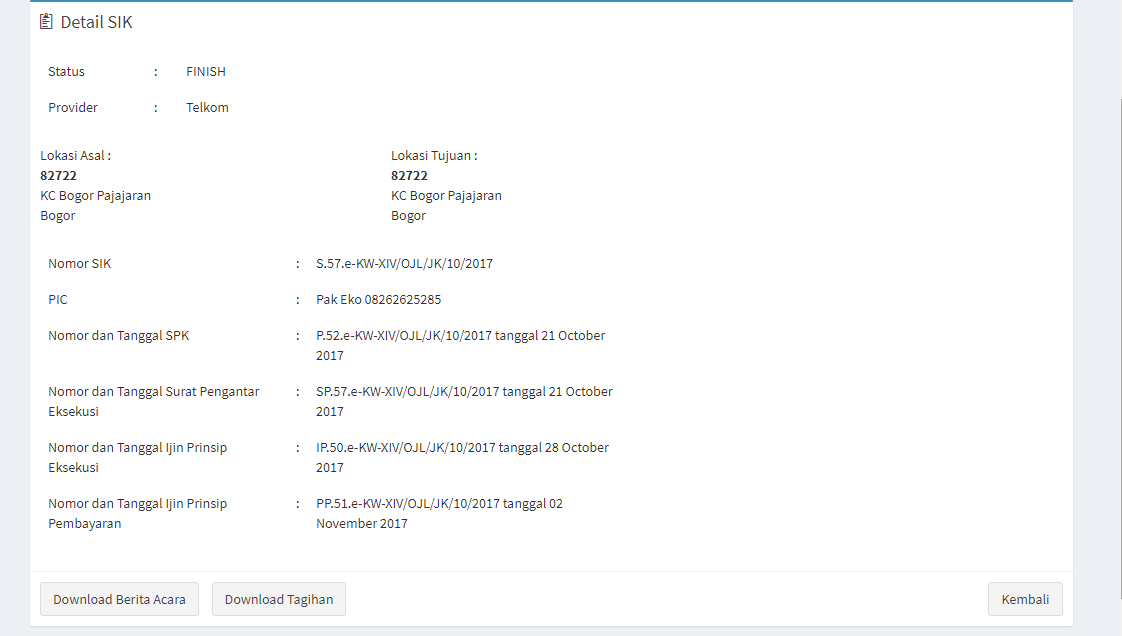
\includegraphics[width=10cm,height=5cm]{bab6/finish.png}}
\caption{Data Detail \textit{Finish}}
\label{figure:data_detail_finish}
\end{figure}

\section{Evaluasi Pengujian}
\tab Hasil pengujian dihasilkan pengamatan lebih lanjut terhadap perilaku sistem \textit{Monitoring} SIK terhadap skenario kasus uji coba. Pengujian dilakukan \textit{internal team} untuk mencoba sistem yang telah diterapkan. Tabel \ref{tab:hasil_pengujian} adalah hasil pengujian pada sistem informasi \textit{monitoring} SIK.
\begin{table}[h!]
	\centering
	\begin{tabular}{|p{6cm}|p{4cm}|}
	\hline
	\textbf{Tugas} & \textbf{Hasil}\\ \hline
	Sistem mampu menampilkan informasi fitur-fitur \textit{Monitoring} SIK & Terpenuhi\\ \hline
	Sistem mampu menampilkan detail informasi kepada user & Terpenuhi\\ \hline
	Sistem mampu menangani pengelolaan data \textit{Monitoring} SIK & Terpenuhi\\ \hline
	Sistem mampu mengeksport data SIK ke dalam bentuk file berekstensi pdf & Terpenuhi\\ \hline
	Sistem menampilkan data sesuai dengan \textit{keyword} pencarian & Terpenuhi\\ \hline
	Sistem dapat mendownload dan upload file ke dalam basis data & Terpenuhi\\ \hline
	\end{tabular}\caption{Hasil Pengujian}
		\label{tab:hasil_pengujian}
\end{table}

Dengan hasil pengujian yang telah dilakukan, dapat disimpulkan bahwa keseluruhan aplikasi \textit{Monitoring} SIK memenuhi kriteria yang disebutkan pada sub-bab sebelumnya.

\section{Evaluasi Performa}
Tabel \ref{tab:evaluasi_performa_1} dan \ref{tab:evaluasi_performa_2} adalah hasil dari uji coba evaluasi performa sistem informasi \textit{monitoring} SIK.
\begin{table}
\centering
\begin{tabular}{|p{5cm}|p{2.5cm}|p{2cm}|}
\hline
\textbf{Tugas} & \textbf{Hasil} & \textbf{Waktu}\\ \hline
Membuka Halaman Dashboard & Terpenuhi & 2 detik\\ \hline
Membuka Halaman Request Relokasi & Terpenuhi & 1 detik\\ \hline
Menambahkan Request Relokasi & Terpenuhi & 2 detik\\ \hline
\end{tabular}\caption{Hasil Uji Performa(1)}
		\label{tab:evaluasi_performa_1}
\end{table}

\begin{table}
\centering
\begin{tabular}{|p{5cm}|p{2.5cm}|p{2cm}|}
\hline
\textbf{Tugas} & \textbf{Hasil} & \textbf{Waktu}\\ \hline
Membuka Halaman SIK & Terpenuhi & 1 detik\\ \hline
Menambahkan SIK & Terpenuhi & 2 detik\\ \hline
Membuka Halaman Penagihan & Terpenuhi & 1 detik\\ \hline
Menambahkan Penagihan & Terpenuhi & 2 detik\\ \hline
Membuka Halaman Eksekusi & Terpenuhi & 1 detik\\ \hline
Menambahkan Eksekusi & Terpenuhi & 2 detik\\ \hline
Membuka Halaman Finish & Terpenuhi & 1 detik\\ \hline
Menambahkan Finish & Terpenuhi & 2 detik\\ \hline
Mendownload Request Relokasi & Terpenuhi & 2 detik\\ \hline
Mendownload SIK & Terpenuhi & 2 detik\\ \hline
Mendownload Berita Acara & Terpenuhi & 2 detik\\ \hline
Mendownload Penagihan & Terpenuhi & 2 detik\\ \hline
\end{tabular}\caption{Hasil Uji Performa(2)}
		\label{tab:evaluasi_performa_2}
\end{table}

\vspace{4 cm}
\textcolor{white}{..}
	\chapter{KESIMPULAN DAN SARAN}

\section{Kesimpulan}
\tab Kesimpulan yang didapat setelah melakukan pengembangan sistem EasyMeeting pada kegiatan Kerja Praktik di PT. Telekomunikasi Indonesia adalah sebagai berikut:
\begin{enumerate}
\item \sistem berhasil dibuat menggunakan Arduino UNO, Telegram Bot API, dan bahasa pemrograman C untuk meningkatkan efisiensi persiapan ruang rapat di PT. Telekomunikasi Indonesia.
\item \sistem dapat membantu meningkatkan pengembangan \textit{Internet of Things} (IoT) di PT. Telekomunikasi Indonesia.
\item \sistem berhasil dibuat sesuai dengan analisis dan perancangan sistem, serta memenuhi kebutuhan fungsional dan non-fungsional PT. Telekomunikasi Indonesia.
\end{enumerate}

\section{Saran}
Setelah melalui Kerja Praktik kali ini, penulis memberikan saran sebagai berikut:
\begin{enumerate}
\item Mikrokontroler Arduino UNO dan ESP8266-01 dapat diganti dengan mikrokontroler NodeMCU (board Arduino sekaligus ESP8266 yang telah ter-\textit{package} menjadi satu) supaya koneksi Wi-Fi pada sirkuit menjadi lebih stabil.
\item Perlu dilakukan penelitian lagi terhadap WSO2 IoT Server.
\end{enumerate}
	
	\appendix
	\begin{thebibliography}{9}
	
	\bibitem{profil-telkom}
	Telkom Indonesia. (n.d.). \textit{Profil dan Riwayat Singkat}. Diakses pada 19 Juni 2018, dari  https://www.telkom.co.id/ servlet/tk/about/id\_ID/stocklanding/profil-dan-riwayat-singkat.html
	
	\bibitem{citekey}
	Telkom Indonesia. (2017, 11 Oktober). \textit{SOA : Untying the Knot, Information Technology Division} [powerpoint slides]. Teks tidak terpublikasi, Telkom Indonesia, Jakarta Selatan, DKI Jakarta, Indonesia. 
	
	\bibitem{citekey}
	Telkom Indonesia [image]. (2015, 19 Desember). Diakses pada 19 Juni 2018, dari https://upload.wikimedia.org/wikipedia/ commons/8/8f/Operator\_Telekomunikasi\_Telkom\_Indonesia.jpg
	
	\bibitem{citekey}
	Kilas Balik Telkom Indonesia \#1 [image] (n.d.). Diakses pada 19 Juni 2018 dari https://konten.telkom.co.id/cs/groups/ cem/documents/digitalmedia/wcc009409.jpg
	
	\bibitem{ashton}
	Ashton, K. (2009, 22 Juni). That 'Internet of Things' Thing. \textit{RFID Journal}. Diakses pada 22 Juni 2018, dari http://www.rfidjournal.com/articles/view?4986
	
	\bibitem{citekey}
	Janssen, D. \& Janssen, C. (n.d.). \textit{Internet of Things (IoT)}. Diakses pada 22 Juni 2018, dari https://www.techopedia.com/definition/28247/internet-of-things-iot
	
	\bibitem{citekey}
	Telegram. (n.d.). \textit{Telegram APIs}. Diakses pada 23 juni 2018, dari https://core.telegram.org/api
	
	\bibitem{citekey}
	Telegram Team. (2015). \textit{Telegram Bot Platform}. Diakses pada 23 juni 2018, dari https://telegram.org/blog/bot-revolution
	
	\bibitem{}
	Cokrojoyo, A., Andjarwirawan, J., \&  Noertjahyana, A. (2017). Pembuatan Bot Telegram Untuk Mengambil Informasi dan Jadwal Film Menggunakan PHP. \textit{Jurnal Infra}, \textit{Universitas Kristen Petra}, \textit{5} (1). Diakses pada 23 Juni 2018, dari https://media.neliti.com/media/publications/ 103478-ID-pembuatan-bot-telegram-untuk-mengambil-i.pdf
	
	http://eprints.akakom.ac.id/4913/3/3\_143310004\_BAB\_II.pdf
	
	http://eprints.akakom.ac.id/4914/3/3\_143310009\_BAB\_ll.pdf 
	
	http://www.handsontec.com/pdf\_learn/esp8266-V10.pdf
	
	https://github.com/nodemcu/nodemcu-devkit
	
	https://embeddednesia.com/v1/?p=2050
\end{thebibliography}

	\backmatter
	\chapter{BIODATA PENULIS}
\begin{wrapfigure}{l}{0.4\textwidth}
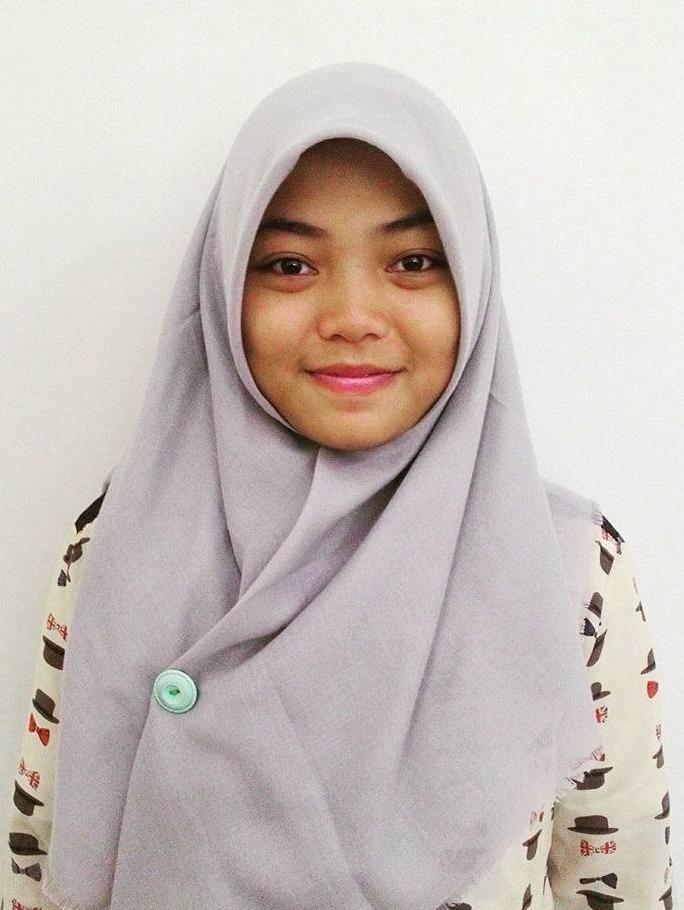
\includegraphics[height=0.3\textheight]{biodata/foto.jpg}
\end{wrapfigure}

\textbf{Desy Nurbaiti Rahmi}, lahir di Banyuwangi tanggal 9 Desember 1995. Penulis merupakan anak ketiga dari 3 bersaudara. Penulis telah menempuh pendidikan formal TK Aisyiyah I Banyuwangi, SD Negeri 1 Kebalenan (2002-2008), SMP Negeri 1 Banyuwangi (2008-2011) dan SMA Negeri 1 Glagah (2011-2014). Penulis melanjutkan studi kuliah program sarjana di Jurusan Teknik Informatika ITS. 

Selama kuliah di Teknik Informatika ITS, penulis  pernah menjadi asisten dosen dan praktikum untuk mata kuliah Sistem Operasi (2016 dan 2017), Jaringan Komputer(2016). Selama menempuh perkuliahan penulis juga aktif di kegiatan organisasi dan kepanitiaan diantaranya menjadi staff Departemen Pengembangan Profesi HMTC ITS, wakil dua Bendahara Schematics 2015, Bendahara Schematics 2015 dan panitia Pemusatan Latihan Nasional 2 TOKI 2017 di ITS. Penulis dapat dihubungi melalui surel di \\ \texttt{desyrahmi09@gmail.com}.

\end{document}
